% Template for ASRU-2017 paper; to be used with:
%          spconf.sty  - ICASSP/ICIP LaTeX style file, and
%          IEEEbib.bst - IEEE bibliography style file.
% --------------------------------------------------------------------------
\documentclass{article}
\usepackage{spconf,amsmath,graphicx}
\usepackage{amssymb,amsmath,bm}
\usepackage{textcomp}
\usepackage{algorithm}
\usepackage{algpseudocode}
\usepackage{float}
\usepackage{multirow}
\usepackage[justification=centering]{caption}
\usepackage[caption = false]{subfig}

% Custom settings

\usepackage{tikz,placeins}
\usetikzlibrary{arrows,decorations.markings}
\tikzstyle{every picture}+=[font=\rmfamily\it\bfseries\large]
\usetikzlibrary{positioning, shapes}
%\usepackage{xcolor} %already loaded by tikz
%
\pgfdeclarelayer{background}
\pgfdeclarelayer{foreground}
\pgfsetlayers{background,main,foreground}


\graphicspath{{../figures/}}


\newcommand{\specialcell}[2][c]{%
     \begin{tabular}[#1]{@{}c@{}}#2\end{tabular}}



\newcommand{\chanwcom}{{C. Kim}}
\renewcommand{\topfraction}{1.0}
\renewcommand{\bottomfraction}{1.0}
\renewcommand{\textfraction}{0.01}
\renewcommand{\floatpagefraction}{1.0}
\renewcommand{\dbltopfraction}{1.0}
\renewcommand{\floatpagefraction}{1.0}  % require fuller float pages
\renewcommand{\dblfloatpagefraction}{1.0} % require fuller float pages
\newcommand{\AR}[1]{{\color{red} arunnt@ COMMENT: #1}}

\ninept


% Example definitions.
% --------------------
\def\x{{\mathbf x}}
\def\L{{\cal L}}

% Title.
% ------
\title{Efficient Implementation of the Room Simulator \\ for Training Deep Neural Network Acoustic Models}
%
% Single address.
% ---------------
\name{{Chanwoo Kim, Ehsan Variani, Arun Narayanan, and Michiel Bacchiani}}

\address{Google Speech \\
%  {\small \tt \{chanwcom, tsainath, arunnt, misra, rnongpiur, michiel\}@google.com }}
  {\small \tt \{chanwcom, variani, arunnt, michiel\}@google.com }}
%
% For example:
% ------------
%\address{School\\
%	Department\\
%	Address}
%
% Two addresses (uncomment and modify for two-address case).
% ----------------------------------------------------------
%\twoauthors
%  {A. Author-one, B. Author-two\sthanks{Thanks to XYZ agency for funding.}}
%	{School A-B\\
%	Department A-B\\
%	Address A-B}
%  {C. Author-three, D. Author-four\sthanks{The fourth author performed the work
%	while at ...}}
%	{School C-D\\
%	Department C-D\\
%	Address C-D}
%
\begin{document}
%
\maketitle
%
\begin{abstract}
In this paper, we describe how to efficiently implement
an acoustic room simulator to generate large-scale
simulated data for training deep neural networks.
Even though the \textit{Room Simulator} in \cite{C_Kim_INTERSPEECH_2017_1} was shown
 to be quite effective in reducing the Word
Error Rates (WERs) for far-field applications by generating
simulated far-field training sets, it requires
high dimensional Fast Fourier Transforms (FFTs).
\textit{Room Simulator} in \cite{C_Kim_INTERSPEECH_2017_1} used 
  approximately 80 percent of CPU usage in our CPU/GPU
training architecture. In this work, we implement an efficient OverLap
  Addition (OLA) based filtering using the open-source \texttt{FFTW3}
library. Further, we investigate the effects of the Room
Impulse Response (RIR) lengths. Experimentally, we conclude that we can cut
the tail portions of RIRs whose power is less than 20 \textit{dB}
below the maximum power without sacrificing the speech recognition accuracy.
Using these approaches, we were able to reduce CPU usage for the
room simulator portion down to 9.69 \%
in CPU/GPU training architecture. Profiling result shows that
we obtain 22.4 times speed-up on a single machine and 37.3 times
  speed up on Google's distributed training infrastructure.
\AR{I don't think we should use borg to describe clusters since it's not something known externally.}
 \end{abstract}
%
\begin{keywords}
Simulated data, room acoustics, robust speech recognition, deep learning
\end{keywords}
%
%
\section{Introduction}
With advancements in deep learning,
\cite{Seltzer2013DNNAurora4, Yu2013FeatureLearningDNN, V_Vanhoucke_Deep_Learning_NIPS_Workshop_2011,
G_Hinton_IEEE_Signal_Process_Mag_2012,
T_Sainath_IEEETran_2017_1, T_Sainath_Book_Chapter_2017_1},
speech recognition accuracy has improved dramatically.
Now, speech recognition systems
are used not only on portable devices
but also on standalone devices for far-field speech recognition.
Examples include voice assistant systems such as Amazon Alexa
and Google Home \cite{C_Kim_INTERSPEECH_2017_1, B_Li_INTERSPEECH_2017_1}.
In far-field speech recognition, the impact of noise and reverberation
is much larger than near-field cases. Traditional approaches to far-field
speech recognition include noise robust feature extraction algorithms
\cite{C_Kim_IEEETran_2016_1, U_H_Yapanel_SpeechComm_2008},
on-set enhancement algorithms
\cite{C_Kim_INTERSPEECH_2010_2, C_Kim_INTERSPEECH_2014_2} \AR{Classification seems too narrow!}.
\AR{Maybe change: Recently, we observed that -> Several studies have now shown that} Recently, we observed that training with noisy data generated
by a \textit{Room Simulator} \cite{C_Kim_INTERSPEECH_2017_1}
improves speech recognition accuracy dramatically.
This system has been successfully employed
for training acoustic models for Google Home or Google voice
search \cite{C_Kim_INTERSPEECH_2017_1}.

\textit{Room Simulator} creates millions of virtual rooms
with different dimensions and different number of sound sources
at different locations and Signal-to-Noise Ratios (SNRs).
For every new utterance in the training set, we use a randomly
sampled room configuration, so that the same utterance
is simulated under different acoustic environments in every epoch during training.
As will be seen in Sec. \ref{sec:experimental_results}, if
we generate the simulated utterance only once for each
input example, the performance is worse.
Since different RIRs are applied for the same
utterance at every epoch, the intermediate results cannot be cached.
Therefore, the noisification process requires several large convolution operations. As will be seen
in Sec. \ref{sec:experimental_results}, during training, it uses up to 80 \%
of the whole CPU usage if we use the CPU/GPU architecture
shown in Fig. \ref{fig:gpu_cpu_structure}.

In this paper, we describe our approach to reduce the
computational cost of the \textit{Room Simulator}. We
first switch from \texttt{Kiss FFT} in
\texttt{Eigen3} to Real FFT in \texttt{FFTW3}. Then we
investigate the required length of RIRs for robust
speech recognition.
%As will be seen in Sec.
%\ref{sec:experimental_results}, we observe that we can remove
%the tail portion or an RIR whose power is 20-dB below
%the maximum power of the original RIR.
%This approach reduced the RIR length to 47 \% compared to the
%original RIR length.
%Combined with OLA filtering, on a local machine, the speed-up
%was 25.2 times. On Google Borg, the speed up was 37.3 times.
%
%
%
%
%
\begin{figure}%[!tbp]
  \begin{center}
    \resizebox{85mm}{!}{% Graphic for TeX using PGF
% Title: /google/src/cloud/chanwcom/chanwcom-speech9999/google3/experimental/users/chanwcom/my_papers/papers_working/room_simulator_comp_reduction_icassp_2018/figures/gpu_cpu_structure.dia
% Creator: Dia v0.97.2
% CreationDate: Wed Nov  8 09:58:56 2017
% For: chanwcom
% \usepackage{tikz}
% The following commands are not supported in PSTricks at present
% We define them conditionally, so when they are implemented,
% this pgf file will use them.
\ifx\du\undefined
  \newlength{\du}
\fi
\setlength{\du}{15\unitlength}
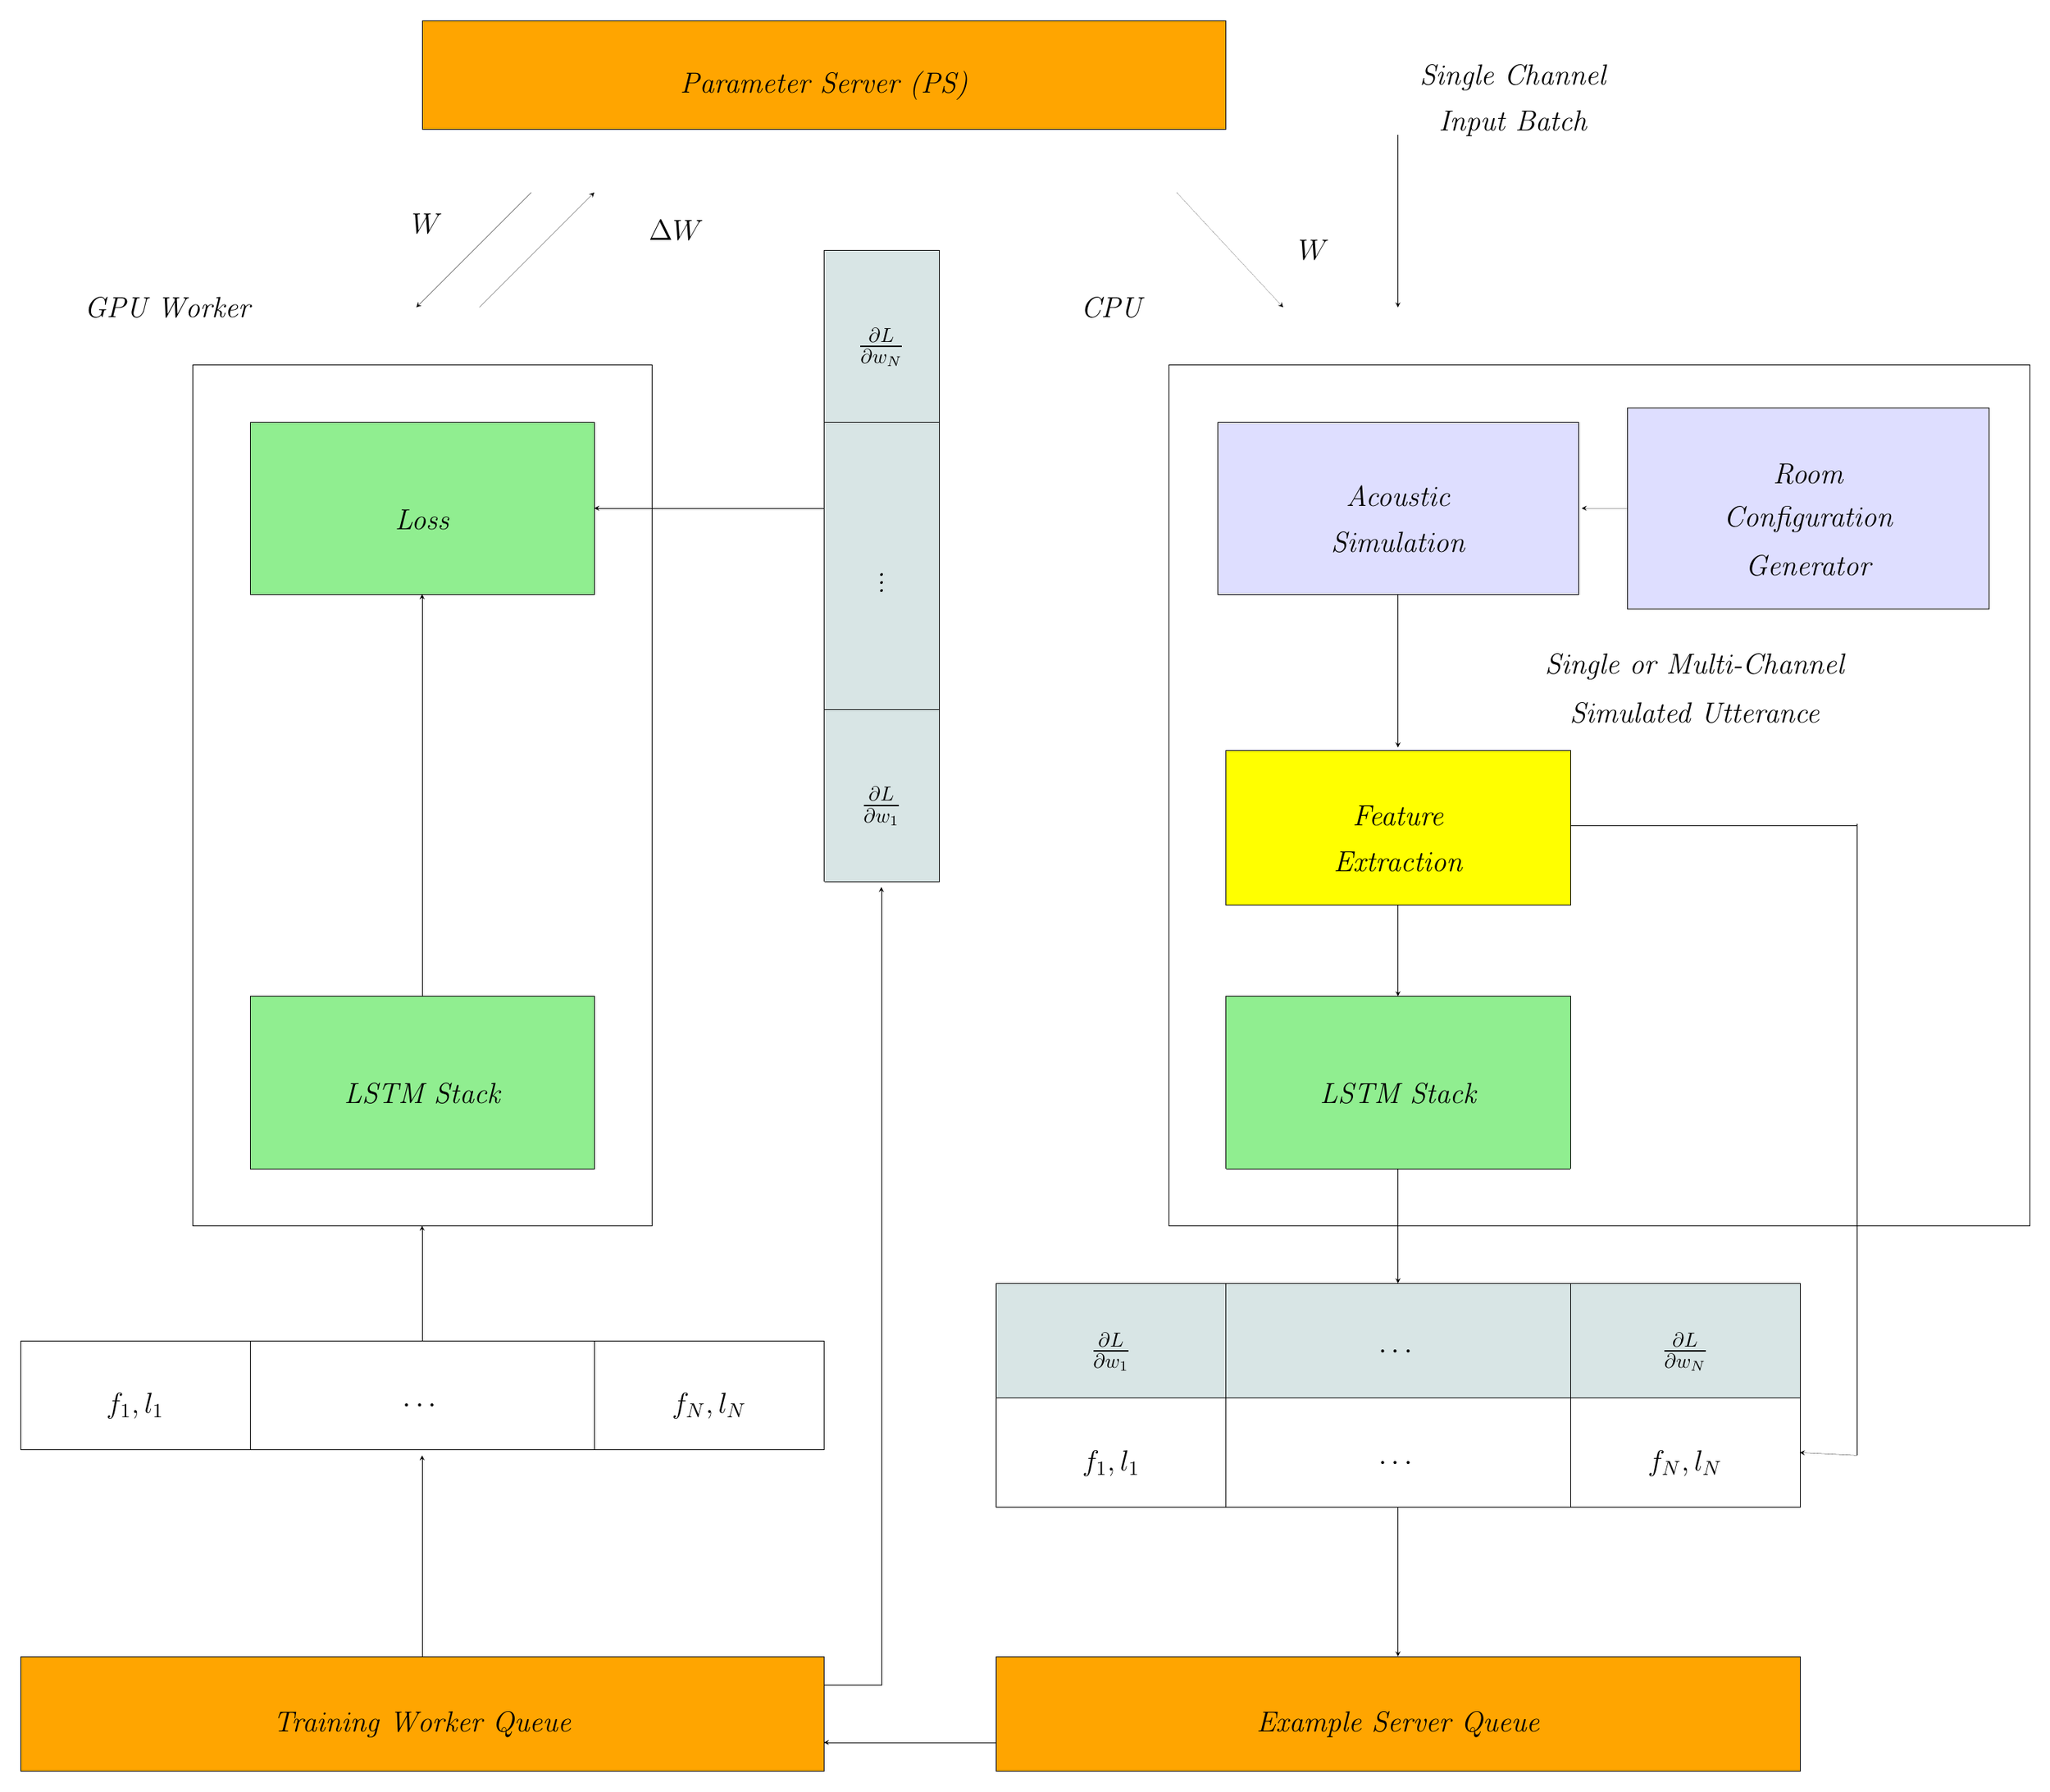
\begin{tikzpicture}
  \tikzstyle{every node}=[font=\Large\itshape]
\pgftransformxscale{1.000000}
\pgftransformyscale{-1.000000}
\definecolor{dialinecolor}{rgb}{0.000000, 0.000000, 0.000000}
\pgfsetstrokecolor{dialinecolor}
\definecolor{dialinecolor}{rgb}{1.000000, 1.000000, 1.000000}
\pgfsetfillcolor{dialinecolor}
\definecolor{dialinecolor}{rgb}{1.000000, 1.000000, 1.000000}
\pgfsetfillcolor{dialinecolor}
\fill (11.000000\du,11.000000\du)--(11.000000\du,26.000000\du)--(19.000000\du,26.000000\du)--(19.000000\du,11.000000\du)--cycle;
\pgfsetlinewidth{0.100000\du}
\pgfsetdash{}{0pt}
\pgfsetdash{}{0pt}
\pgfsetmiterjoin
\definecolor{dialinecolor}{rgb}{0.000000, 0.000000, 0.000000}
\pgfsetstrokecolor{dialinecolor}
\draw (11.000000\du,11.000000\du)--(11.000000\du,26.000000\du)--(19.000000\du,26.000000\du)--(19.000000\du,11.000000\du)--cycle;
% setfont left to latex
\definecolor{dialinecolor}{rgb}{0.000000, 0.000000, 0.000000}
\pgfsetstrokecolor{dialinecolor}
\node at (15.000000\du,18.695000\du){};
% setfont left to latex
\definecolor{dialinecolor}{rgb}{0.000000, 0.000000, 0.000000}
\pgfsetstrokecolor{dialinecolor}
\node[anchor=west] at (9.000000\du,10.000000\du){GPU Worker};
\definecolor{dialinecolor}{rgb}{0.564706, 0.933333, 0.564706}
\pgfsetfillcolor{dialinecolor}
\fill (12.000000\du,12.000000\du)--(12.000000\du,15.000000\du)--(18.000000\du,15.000000\du)--(18.000000\du,12.000000\du)--cycle;
\pgfsetlinewidth{0.100000\du}
\pgfsetdash{}{0pt}
\pgfsetdash{}{0pt}
\pgfsetmiterjoin
\definecolor{dialinecolor}{rgb}{0.000000, 0.000000, 0.000000}
\pgfsetstrokecolor{dialinecolor}
\draw (12.000000\du,12.000000\du)--(12.000000\du,15.000000\du)--(18.000000\du,15.000000\du)--(18.000000\du,12.000000\du)--cycle;
% setfont left to latex
\definecolor{dialinecolor}{rgb}{0.000000, 0.000000, 0.000000}
\pgfsetstrokecolor{dialinecolor}
\node at (15.000000\du,13.695000\du){Loss};
\definecolor{dialinecolor}{rgb}{0.564706, 0.933333, 0.564706}
\pgfsetfillcolor{dialinecolor}
\fill (12.000000\du,22.000000\du)--(12.000000\du,25.000000\du)--(18.000000\du,25.000000\du)--(18.000000\du,22.000000\du)--cycle;
\pgfsetlinewidth{0.100000\du}
\pgfsetdash{}{0pt}
\pgfsetdash{}{0pt}
\pgfsetmiterjoin
\definecolor{dialinecolor}{rgb}{0.000000, 0.000000, 0.000000}
\pgfsetstrokecolor{dialinecolor}
\draw (12.000000\du,22.000000\du)--(12.000000\du,25.000000\du)--(18.000000\du,25.000000\du)--(18.000000\du,22.000000\du)--cycle;
% setfont left to latex
\definecolor{dialinecolor}{rgb}{0.000000, 0.000000, 0.000000}
\pgfsetstrokecolor{dialinecolor}
\node at (15.000000\du,23.695000\du){LSTM Stack};
\pgfsetlinewidth{0.100000\du}
\pgfsetdash{}{0pt}
\pgfsetdash{}{0pt}
\pgfsetbuttcap
{
\definecolor{dialinecolor}{rgb}{0.000000, 0.000000, 0.000000}
\pgfsetfillcolor{dialinecolor}
% was here!!!
\pgfsetarrowsend{stealth}
\definecolor{dialinecolor}{rgb}{0.000000, 0.000000, 0.000000}
\pgfsetstrokecolor{dialinecolor}
\draw (16.000000\du,10.000000\du)--(18.000000\du,8.000000\du);
}
\definecolor{dialinecolor}{rgb}{1.000000, 1.000000, 1.000000}
\pgfsetfillcolor{dialinecolor}
\fill (28.000300\du,11.000000\du)--(28.000300\du,26.000000\du)--(43.000000\du,26.000000\du)--(43.000000\du,11.000000\du)--cycle;
\pgfsetlinewidth{0.100000\du}
\pgfsetdash{}{0pt}
\pgfsetdash{}{0pt}
\pgfsetmiterjoin
\definecolor{dialinecolor}{rgb}{0.000000, 0.000000, 0.000000}
\pgfsetstrokecolor{dialinecolor}
\draw (28.000300\du,11.000000\du)--(28.000300\du,26.000000\du)--(43.000000\du,26.000000\du)--(43.000000\du,11.000000\du)--cycle;
% setfont left to latex
\definecolor{dialinecolor}{rgb}{0.000000, 0.000000, 0.000000}
\pgfsetstrokecolor{dialinecolor}
\node at (35.500150\du,18.695000\du){};
\definecolor{dialinecolor}{rgb}{1.000000, 1.000000, 0.000000}
\pgfsetfillcolor{dialinecolor}
\fill (29.000300\du,17.713508\du)--(29.000300\du,20.413508\du)--(35.000300\du,20.413508\du)--(35.000300\du,17.713508\du)--cycle;
\pgfsetlinewidth{0.100000\du}
\pgfsetdash{}{0pt}
\pgfsetdash{}{0pt}
\pgfsetmiterjoin
\definecolor{dialinecolor}{rgb}{0.000000, 0.000000, 0.000000}
\pgfsetstrokecolor{dialinecolor}
\draw (29.000300\du,17.713508\du)--(29.000300\du,20.413508\du)--(35.000300\du,20.413508\du)--(35.000300\du,17.713508\du)--cycle;
% setfont left to latex
\definecolor{dialinecolor}{rgb}{0.000000, 0.000000, 0.000000}
\pgfsetstrokecolor{dialinecolor}
\node at (32.000300\du,18.858508\du){Feature};
% setfont left to latex
\definecolor{dialinecolor}{rgb}{0.000000, 0.000000, 0.000000}
\pgfsetstrokecolor{dialinecolor}
\node at (32.000300\du,19.658508\du){Extraction};
\definecolor{dialinecolor}{rgb}{0.564706, 0.933333, 0.564706}
\pgfsetfillcolor{dialinecolor}
\fill (29.000300\du,22.000000\du)--(29.000300\du,25.000000\du)--(35.000300\du,25.000000\du)--(35.000300\du,22.000000\du)--cycle;
\pgfsetlinewidth{0.100000\du}
\pgfsetdash{{\pgflinewidth}{0.200000\du}}{0cm}
\pgfsetdash{{\pgflinewidth}{0.200000\du}}{0cm}
\pgfsetmiterjoin
\definecolor{dialinecolor}{rgb}{0.000000, 0.000000, 0.000000}
\pgfsetstrokecolor{dialinecolor}
\draw (29.000300\du,22.000000\du)--(29.000300\du,25.000000\du)--(35.000300\du,25.000000\du)--(35.000300\du,22.000000\du)--cycle;
% setfont left to latex
\definecolor{dialinecolor}{rgb}{0.000000, 0.000000, 0.000000}
\pgfsetstrokecolor{dialinecolor}
\node at (32.000300\du,23.695000\du){LSTM Stack};
\pgfsetlinewidth{0.100000\du}
\pgfsetdash{{\pgflinewidth}{0.200000\du}}{0cm}
\pgfsetdash{{\pgflinewidth}{0.200000\du}}{0cm}
\pgfsetbuttcap
{
\definecolor{dialinecolor}{rgb}{0.000000, 0.000000, 0.000000}
\pgfsetfillcolor{dialinecolor}
% was here!!!
\pgfsetarrowsend{stealth}
\definecolor{dialinecolor}{rgb}{0.000000, 0.000000, 0.000000}
\pgfsetstrokecolor{dialinecolor}
\draw (32.000300\du,20.413508\du)--(32.000300\du,22.000000\du);
}
% setfont left to latex
\definecolor{dialinecolor}{rgb}{0.000000, 0.000000, 0.000000}
\pgfsetstrokecolor{dialinecolor}
\node[anchor=west] at (32.000300\du,19.063508\du){};
\definecolor{dialinecolor}{rgb}{1.000000, 0.647059, 0.000000}
\pgfsetfillcolor{dialinecolor}
\fill (15.000000\du,5.000000\du)--(15.000000\du,6.900000\du)--(29.000000\du,6.900000\du)--(29.000000\du,5.000000\du)--cycle;
\pgfsetlinewidth{0.100000\du}
\pgfsetdash{}{0pt}
\pgfsetdash{}{0pt}
\pgfsetmiterjoin
\definecolor{dialinecolor}{rgb}{0.000000, 0.000000, 0.000000}
\pgfsetstrokecolor{dialinecolor}
\draw (15.000000\du,5.000000\du)--(15.000000\du,6.900000\du)--(29.000000\du,6.900000\du)--(29.000000\du,5.000000\du)--cycle;
% setfont left to latex
\definecolor{dialinecolor}{rgb}{0.000000, 0.000000, 0.000000}
\pgfsetstrokecolor{dialinecolor}
\node at (22.000000\du,6.145000\du){Parameter Server (PS)};
% setfont left to latex
\definecolor{dialinecolor}{rgb}{0.000000, 0.000000, 0.000000}
\pgfsetstrokecolor{dialinecolor}
\node[anchor=west] at (22.000000\du,5.950000\du){};
% setfont left to latex
\definecolor{dialinecolor}{rgb}{0.000000, 0.000000, 0.000000}
\pgfsetstrokecolor{dialinecolor}
\node[anchor=west] at (22.000000\du,5.950000\du){};
\pgfsetlinewidth{0.100000\du}
\pgfsetdash{{\pgflinewidth}{0.200000\du}}{0cm}
\pgfsetdash{{\pgflinewidth}{0.200000\du}}{0cm}
\pgfsetbuttcap
{
\definecolor{dialinecolor}{rgb}{0.000000, 0.000000, 0.000000}
\pgfsetfillcolor{dialinecolor}
% was here!!!
\pgfsetarrowsend{stealth}
\definecolor{dialinecolor}{rgb}{0.000000, 0.000000, 0.000000}
\pgfsetstrokecolor{dialinecolor}
\draw (28.144500\du,8.000000\du)--(30.000000\du,10.000000\du);
}
\definecolor{dialinecolor}{rgb}{0.870588, 0.870588, 1.000000}
\pgfsetfillcolor{dialinecolor}
\fill (28.855300\du,12.000000\du)--(28.855300\du,15.000000\du)--(35.145300\du,15.000000\du)--(35.145300\du,12.000000\du)--cycle;
\pgfsetlinewidth{0.100000\du}
\pgfsetdash{}{0pt}
\pgfsetdash{}{0pt}
\pgfsetmiterjoin
\definecolor{dialinecolor}{rgb}{0.000000, 0.000000, 0.000000}
\pgfsetstrokecolor{dialinecolor}
\draw (28.855300\du,12.000000\du)--(28.855300\du,15.000000\du)--(35.145300\du,15.000000\du)--(35.145300\du,12.000000\du)--cycle;
% setfont left to latex
\definecolor{dialinecolor}{rgb}{0.000000, 0.000000, 0.000000}
\pgfsetstrokecolor{dialinecolor}
\node at (32.000300\du,13.295000\du){Acoustic };
% setfont left to latex
\definecolor{dialinecolor}{rgb}{0.000000, 0.000000, 0.000000}
\pgfsetstrokecolor{dialinecolor}
\node at (32.000300\du,14.095000\du){Simulation};
\pgfsetlinewidth{0.100000\du}
\pgfsetdash{}{0pt}
\pgfsetdash{}{0pt}
\pgfsetbuttcap
{
\definecolor{dialinecolor}{rgb}{0.000000, 0.000000, 0.000000}
\pgfsetfillcolor{dialinecolor}
% was here!!!
\pgfsetarrowsend{stealth}
\definecolor{dialinecolor}{rgb}{0.000000, 0.000000, 0.000000}
\pgfsetstrokecolor{dialinecolor}
\draw (16.900000\du,8.000000\du)--(14.900000\du,10.000000\du);
}
\definecolor{dialinecolor}{rgb}{1.000000, 0.647059, 0.000000}
\pgfsetfillcolor{dialinecolor}
\fill (8.000000\du,33.500000\du)--(8.000000\du,35.500000\du)--(22.000000\du,35.500000\du)--(22.000000\du,33.500000\du)--cycle;
\pgfsetlinewidth{0.100000\du}
\pgfsetdash{}{0pt}
\pgfsetdash{}{0pt}
\pgfsetmiterjoin
\definecolor{dialinecolor}{rgb}{0.000000, 0.000000, 0.000000}
\pgfsetstrokecolor{dialinecolor}
\draw (8.000000\du,33.500000\du)--(8.000000\du,35.500000\du)--(22.000000\du,35.500000\du)--(22.000000\du,33.500000\du)--cycle;
% setfont left to latex
\definecolor{dialinecolor}{rgb}{0.000000, 0.000000, 0.000000}
\pgfsetstrokecolor{dialinecolor}
\node at (15.000000\du,34.695000\du){Training Worker Queue};
\pgfsetlinewidth{0.100000\du}
\pgfsetdash{}{0pt}
\pgfsetdash{}{0pt}
\pgfsetbuttcap
{
\definecolor{dialinecolor}{rgb}{0.000000, 0.000000, 0.000000}
\pgfsetfillcolor{dialinecolor}
% was here!!!
\pgfsetarrowsend{stealth}
\definecolor{dialinecolor}{rgb}{0.000000, 0.000000, 0.000000}
\pgfsetstrokecolor{dialinecolor}
\draw (15.000000\du,33.500000\du)--(15.000000\du,30.000000\du);
}
\pgfsetlinewidth{0.100000\du}
\pgfsetdash{}{0pt}
\pgfsetdash{}{0pt}
\pgfsetbuttcap
{
\definecolor{dialinecolor}{rgb}{0.000000, 0.000000, 0.000000}
\pgfsetfillcolor{dialinecolor}
% was here!!!
\pgfsetarrowsend{stealth}
\definecolor{dialinecolor}{rgb}{0.000000, 0.000000, 0.000000}
\pgfsetstrokecolor{dialinecolor}
\draw (15.000000\du,28.000000\du)--(15.000000\du,26.000000\du);
}
\definecolor{dialinecolor}{rgb}{1.000000, 1.000000, 1.000000}
\pgfsetfillcolor{dialinecolor}
\fill (8.000000\du,28.000000\du)--(8.000000\du,29.900000\du)--(12.000000\du,29.900000\du)--(12.000000\du,28.000000\du)--cycle;
\pgfsetlinewidth{0.100000\du}
\pgfsetdash{}{0pt}
\pgfsetdash{}{0pt}
\pgfsetmiterjoin
\definecolor{dialinecolor}{rgb}{0.000000, 0.000000, 0.000000}
\pgfsetstrokecolor{dialinecolor}
\draw (8.000000\du,28.000000\du)--(8.000000\du,29.900000\du)--(12.000000\du,29.900000\du)--(12.000000\du,28.000000\du)--cycle;
% setfont left to latex
\definecolor{dialinecolor}{rgb}{0.000000, 0.000000, 0.000000}
\pgfsetstrokecolor{dialinecolor}
\node at (10.000000\du,29.145000\du){$f_1, l_1$};
\definecolor{dialinecolor}{rgb}{1.000000, 1.000000, 1.000000}
\pgfsetfillcolor{dialinecolor}
\fill (18.000000\du,28.000000\du)--(18.000000\du,29.900000\du)--(22.000000\du,29.900000\du)--(22.000000\du,28.000000\du)--cycle;
\pgfsetlinewidth{0.100000\du}
\pgfsetdash{}{0pt}
\pgfsetdash{}{0pt}
\pgfsetmiterjoin
\definecolor{dialinecolor}{rgb}{0.000000, 0.000000, 0.000000}
\pgfsetstrokecolor{dialinecolor}
\draw (18.000000\du,28.000000\du)--(18.000000\du,29.900000\du)--(22.000000\du,29.900000\du)--(22.000000\du,28.000000\du)--cycle;
% setfont left to latex
\definecolor{dialinecolor}{rgb}{0.000000, 0.000000, 0.000000}
\pgfsetstrokecolor{dialinecolor}
\node at (20.000000\du,29.145000\du){$f_N, l_N$};
\definecolor{dialinecolor}{rgb}{1.000000, 0.647059, 0.000000}
\pgfsetfillcolor{dialinecolor}
\fill (25.000300\du,33.500000\du)--(25.000300\du,35.500000\du)--(39.000300\du,35.500000\du)--(39.000300\du,33.500000\du)--cycle;
\pgfsetlinewidth{0.100000\du}
\pgfsetdash{}{0pt}
\pgfsetdash{}{0pt}
\pgfsetmiterjoin
\definecolor{dialinecolor}{rgb}{0.000000, 0.000000, 0.000000}
\pgfsetstrokecolor{dialinecolor}
\draw (25.000300\du,33.500000\du)--(25.000300\du,35.500000\du)--(39.000300\du,35.500000\du)--(39.000300\du,33.500000\du)--cycle;
% setfont left to latex
\definecolor{dialinecolor}{rgb}{0.000000, 0.000000, 0.000000}
\pgfsetstrokecolor{dialinecolor}
\node at (32.000300\du,34.695000\du){Example Server Queue};
\definecolor{dialinecolor}{rgb}{1.000000, 1.000000, 1.000000}
\pgfsetfillcolor{dialinecolor}
\fill (12.000000\du,28.000000\du)--(12.000000\du,29.900000\du)--(18.000000\du,29.900000\du)--(18.000000\du,28.000000\du)--cycle;
\pgfsetlinewidth{0.100000\du}
\pgfsetdash{}{0pt}
\pgfsetdash{}{0pt}
\pgfsetmiterjoin
\definecolor{dialinecolor}{rgb}{0.000000, 0.000000, 0.000000}
\pgfsetstrokecolor{dialinecolor}
\draw (12.000000\du,28.000000\du)--(12.000000\du,29.900000\du)--(18.000000\du,29.900000\du)--(18.000000\du,28.000000\du)--cycle;
% setfont left to latex
\definecolor{dialinecolor}{rgb}{0.000000, 0.000000, 0.000000}
\pgfsetstrokecolor{dialinecolor}
\node at (15.000000\du,29.145000\du){$\cdots$};
\definecolor{dialinecolor}{rgb}{0.847059, 0.898039, 0.898039}
\pgfsetfillcolor{dialinecolor}
\fill (25.000300\du,27.000000\du)--(25.000300\du,29.000000\du)--(29.000300\du,29.000000\du)--(29.000300\du,27.000000\du)--cycle;
\pgfsetlinewidth{0.100000\du}
\pgfsetdash{{\pgflinewidth}{0.200000\du}}{0cm}
\pgfsetdash{{\pgflinewidth}{0.200000\du}}{0cm}
\pgfsetmiterjoin
\definecolor{dialinecolor}{rgb}{0.000000, 0.000000, 0.000000}
\pgfsetstrokecolor{dialinecolor}
\draw (25.000300\du,27.000000\du)--(25.000300\du,29.000000\du)--(29.000300\du,29.000000\du)--(29.000300\du,27.000000\du)--cycle;
% setfont left to latex
\definecolor{dialinecolor}{rgb}{0.000000, 0.000000, 0.000000}
\pgfsetstrokecolor{dialinecolor}
\node at (27.000300\du,28.195000\du){$\frac{\partial L}{\partial w_1}$};
\definecolor{dialinecolor}{rgb}{0.847059, 0.898039, 0.898039}
\pgfsetfillcolor{dialinecolor}
\fill (35.000300\du,27.000000\du)--(35.000300\du,29.000000\du)--(39.000300\du,29.000000\du)--(39.000300\du,27.000000\du)--cycle;
\pgfsetlinewidth{0.100000\du}
\pgfsetdash{{\pgflinewidth}{0.200000\du}}{0cm}
\pgfsetdash{{\pgflinewidth}{0.200000\du}}{0cm}
\pgfsetmiterjoin
\definecolor{dialinecolor}{rgb}{0.000000, 0.000000, 0.000000}
\pgfsetstrokecolor{dialinecolor}
\draw (35.000300\du,27.000000\du)--(35.000300\du,29.000000\du)--(39.000300\du,29.000000\du)--(39.000300\du,27.000000\du)--cycle;
% setfont left to latex
\definecolor{dialinecolor}{rgb}{0.000000, 0.000000, 0.000000}
\pgfsetstrokecolor{dialinecolor}
\node at (37.000300\du,28.195000\du){$\frac{\partial L}{\partial w_N}$};
\definecolor{dialinecolor}{rgb}{0.847059, 0.898039, 0.898039}
\pgfsetfillcolor{dialinecolor}
\fill (29.000300\du,27.000000\du)--(29.000300\du,29.000000\du)--(35.000300\du,29.000000\du)--(35.000300\du,27.000000\du)--cycle;
\pgfsetlinewidth{0.100000\du}
\pgfsetdash{{\pgflinewidth}{0.200000\du}}{0cm}
\pgfsetdash{{\pgflinewidth}{0.200000\du}}{0cm}
\pgfsetmiterjoin
\definecolor{dialinecolor}{rgb}{0.000000, 0.000000, 0.000000}
\pgfsetstrokecolor{dialinecolor}
\draw (29.000300\du,27.000000\du)--(29.000300\du,29.000000\du)--(35.000300\du,29.000000\du)--(35.000300\du,27.000000\du)--cycle;
% setfont left to latex
\definecolor{dialinecolor}{rgb}{0.000000, 0.000000, 0.000000}
\pgfsetstrokecolor{dialinecolor}
\node at (32.000300\du,28.195000\du){$\cdots$};
\definecolor{dialinecolor}{rgb}{1.000000, 1.000000, 1.000000}
\pgfsetfillcolor{dialinecolor}
\fill (25.000300\du,29.000000\du)--(25.000300\du,30.900000\du)--(29.000300\du,30.900000\du)--(29.000300\du,29.000000\du)--cycle;
\pgfsetlinewidth{0.100000\du}
\pgfsetdash{}{0pt}
\pgfsetdash{}{0pt}
\pgfsetmiterjoin
\definecolor{dialinecolor}{rgb}{0.000000, 0.000000, 0.000000}
\pgfsetstrokecolor{dialinecolor}
\draw (25.000300\du,29.000000\du)--(25.000300\du,30.900000\du)--(29.000300\du,30.900000\du)--(29.000300\du,29.000000\du)--cycle;
% setfont left to latex
\definecolor{dialinecolor}{rgb}{0.000000, 0.000000, 0.000000}
\pgfsetstrokecolor{dialinecolor}
\node at (27.000300\du,30.145000\du){$f_1,l_1$};
\definecolor{dialinecolor}{rgb}{1.000000, 1.000000, 1.000000}
\pgfsetfillcolor{dialinecolor}
\fill (35.000300\du,29.000000\du)--(35.000300\du,30.900000\du)--(39.000300\du,30.900000\du)--(39.000300\du,29.000000\du)--cycle;
\pgfsetlinewidth{0.100000\du}
\pgfsetdash{}{0pt}
\pgfsetdash{}{0pt}
\pgfsetmiterjoin
\definecolor{dialinecolor}{rgb}{0.000000, 0.000000, 0.000000}
\pgfsetstrokecolor{dialinecolor}
\draw (35.000300\du,29.000000\du)--(35.000300\du,30.900000\du)--(39.000300\du,30.900000\du)--(39.000300\du,29.000000\du)--cycle;
% setfont left to latex
\definecolor{dialinecolor}{rgb}{0.000000, 0.000000, 0.000000}
\pgfsetstrokecolor{dialinecolor}
\node at (37.000300\du,30.145000\du){$f_N, l_N$};
\definecolor{dialinecolor}{rgb}{1.000000, 1.000000, 1.000000}
\pgfsetfillcolor{dialinecolor}
\fill (29.000300\du,29.000000\du)--(29.000300\du,30.900000\du)--(35.000300\du,30.900000\du)--(35.000300\du,29.000000\du)--cycle;
\pgfsetlinewidth{0.100000\du}
\pgfsetdash{}{0pt}
\pgfsetdash{}{0pt}
\pgfsetmiterjoin
\definecolor{dialinecolor}{rgb}{0.000000, 0.000000, 0.000000}
\pgfsetstrokecolor{dialinecolor}
\draw (29.000300\du,29.000000\du)--(29.000300\du,30.900000\du)--(35.000300\du,30.900000\du)--(35.000300\du,29.000000\du)--cycle;
% setfont left to latex
\definecolor{dialinecolor}{rgb}{0.000000, 0.000000, 0.000000}
\pgfsetstrokecolor{dialinecolor}
\node at (32.000300\du,30.145000\du){$\cdots$};
\pgfsetlinewidth{0.100000\du}
\pgfsetdash{{\pgflinewidth}{0.200000\du}}{0cm}
\pgfsetdash{{\pgflinewidth}{0.200000\du}}{0cm}
\pgfsetbuttcap
{
\definecolor{dialinecolor}{rgb}{0.000000, 0.000000, 0.000000}
\pgfsetfillcolor{dialinecolor}
% was here!!!
\pgfsetarrowsend{stealth}
\definecolor{dialinecolor}{rgb}{0.000000, 0.000000, 0.000000}
\pgfsetstrokecolor{dialinecolor}
\draw (32.000300\du,25.000000\du)--(32.000300\du,27.000000\du);
}
\pgfsetlinewidth{0.100000\du}
\pgfsetdash{}{0pt}
\pgfsetdash{}{0pt}
\pgfsetbuttcap
{
\definecolor{dialinecolor}{rgb}{0.000000, 0.000000, 0.000000}
\pgfsetfillcolor{dialinecolor}
% was here!!!
\definecolor{dialinecolor}{rgb}{0.000000, 0.000000, 0.000000}
\pgfsetstrokecolor{dialinecolor}
\draw (35.000000\du,19.029730\du)--(40.000000\du,19.029730\du);
}
\pgfsetlinewidth{0.100000\du}
\pgfsetdash{}{0pt}
\pgfsetdash{}{0pt}
\pgfsetbuttcap
{
\definecolor{dialinecolor}{rgb}{0.000000, 0.000000, 0.000000}
\pgfsetfillcolor{dialinecolor}
% was here!!!
\pgfsetarrowsend{stealth}
\definecolor{dialinecolor}{rgb}{0.000000, 0.000000, 0.000000}
\pgfsetstrokecolor{dialinecolor}
\draw (32.000300\du,15.000000\du)--(32.000300\du,17.664693\du);
}
\pgfsetlinewidth{0.100000\du}
\pgfsetdash{}{0pt}
\pgfsetdash{}{0pt}
\pgfsetbuttcap
{
\definecolor{dialinecolor}{rgb}{0.000000, 0.000000, 0.000000}
\pgfsetfillcolor{dialinecolor}
% was here!!!
\definecolor{dialinecolor}{rgb}{0.000000, 0.000000, 0.000000}
\pgfsetstrokecolor{dialinecolor}
\draw (40.000000\du,19.000000\du)--(40.000000\du,30.000000\du);
}
\pgfsetlinewidth{0.100000\du}
\pgfsetdash{}{0pt}
\pgfsetdash{}{0pt}
\pgfsetbuttcap
{
\definecolor{dialinecolor}{rgb}{0.000000, 0.000000, 0.000000}
\pgfsetfillcolor{dialinecolor}
% was here!!!
\pgfsetarrowsend{stealth}
\definecolor{dialinecolor}{rgb}{0.000000, 0.000000, 0.000000}
\pgfsetstrokecolor{dialinecolor}
\draw (32.000300\du,30.900000\du)--(32.000300\du,33.500000\du);
}
\pgfsetlinewidth{0.100000\du}
\pgfsetdash{}{0pt}
\pgfsetdash{}{0pt}
\pgfsetbuttcap
{
\definecolor{dialinecolor}{rgb}{0.000000, 0.000000, 0.000000}
\pgfsetfillcolor{dialinecolor}
% was here!!!
\pgfsetarrowsend{stealth}
\definecolor{dialinecolor}{rgb}{0.000000, 0.000000, 0.000000}
\pgfsetstrokecolor{dialinecolor}
\draw (25.000300\du,35.000000\du)--(22.000000\du,35.000000\du);
}
\pgfsetlinewidth{0.100000\du}
\pgfsetdash{}{0pt}
\pgfsetdash{}{0pt}
\pgfsetbuttcap
{
\definecolor{dialinecolor}{rgb}{0.000000, 0.000000, 0.000000}
\pgfsetfillcolor{dialinecolor}
% was here!!!
\pgfsetarrowsend{stealth}
\definecolor{dialinecolor}{rgb}{0.000000, 0.000000, 0.000000}
\pgfsetstrokecolor{dialinecolor}
\draw (32.000000\du,7.000000\du)--(32.000000\du,10.000000\du);
}
% setfont left to latex
\definecolor{dialinecolor}{rgb}{0.000000, 0.000000, 0.000000}
\pgfsetstrokecolor{dialinecolor}
\node at (34.000000\du,6.000000\du){Single Channel};
% setfont left to latex
\definecolor{dialinecolor}{rgb}{0.000000, 0.000000, 0.000000}
\pgfsetstrokecolor{dialinecolor}
\node at (34.000000\du,6.800000\du){Input Batch};
\pgfsetlinewidth{0.100000\du}
\pgfsetdash{}{0pt}
\pgfsetdash{}{0pt}
\pgfsetbuttcap
{
\definecolor{dialinecolor}{rgb}{0.000000, 0.000000, 0.000000}
\pgfsetfillcolor{dialinecolor}
% was here!!!
\pgfsetarrowsend{stealth}
\definecolor{dialinecolor}{rgb}{0.000000, 0.000000, 0.000000}
\pgfsetstrokecolor{dialinecolor}
\draw (15.000000\du,22.000000\du)--(15.000000\du,15.000000\du);
}
\definecolor{dialinecolor}{rgb}{0.847059, 0.898039, 0.898039}
\pgfsetfillcolor{dialinecolor}
\fill (22.000000\du,17.000000\du)--(22.000000\du,20.000000\du)--(24.000000\du,20.000000\du)--(24.000000\du,17.000000\du)--cycle;
\pgfsetlinewidth{0.100000\du}
\pgfsetdash{{\pgflinewidth}{0.200000\du}}{0cm}
\pgfsetdash{{\pgflinewidth}{0.200000\du}}{0cm}
\pgfsetmiterjoin
\definecolor{dialinecolor}{rgb}{0.000000, 0.000000, 0.000000}
\pgfsetstrokecolor{dialinecolor}
\draw (22.000000\du,17.000000\du)--(22.000000\du,20.000000\du)--(24.000000\du,20.000000\du)--(24.000000\du,17.000000\du)--cycle;
% setfont left to latex
\definecolor{dialinecolor}{rgb}{0.000000, 0.000000, 0.000000}
\pgfsetstrokecolor{dialinecolor}
\node at (23.000000\du,18.695000\du){$\frac{\partial L}{\partial w_1}$};
\definecolor{dialinecolor}{rgb}{0.847059, 0.898039, 0.898039}
\pgfsetfillcolor{dialinecolor}
\fill (22.000000\du,12.000000\du)--(22.000000\du,17.000000\du)--(24.000000\du,17.000000\du)--(24.000000\du,12.000000\du)--cycle;
\pgfsetlinewidth{0.100000\du}
\pgfsetdash{{\pgflinewidth}{0.200000\du}}{0cm}
\pgfsetdash{{\pgflinewidth}{0.200000\du}}{0cm}
\pgfsetmiterjoin
\definecolor{dialinecolor}{rgb}{0.000000, 0.000000, 0.000000}
\pgfsetstrokecolor{dialinecolor}
\draw (22.000000\du,12.000000\du)--(22.000000\du,17.000000\du)--(24.000000\du,17.000000\du)--(24.000000\du,12.000000\du)--cycle;
% setfont left to latex
\definecolor{dialinecolor}{rgb}{0.000000, 0.000000, 0.000000}
\pgfsetstrokecolor{dialinecolor}
\node at (23.000000\du,14.695000\du){$\vdots$};
\definecolor{dialinecolor}{rgb}{0.847059, 0.898039, 0.898039}
\pgfsetfillcolor{dialinecolor}
\fill (22.000000\du,9.000000\du)--(22.000000\du,12.000000\du)--(24.000000\du,12.000000\du)--(24.000000\du,9.000000\du)--cycle;
\pgfsetlinewidth{0.100000\du}
\pgfsetdash{{\pgflinewidth}{0.200000\du}}{0cm}
\pgfsetdash{{\pgflinewidth}{0.200000\du}}{0cm}
\pgfsetmiterjoin
\definecolor{dialinecolor}{rgb}{0.000000, 0.000000, 0.000000}
\pgfsetstrokecolor{dialinecolor}
\draw (22.000000\du,9.000000\du)--(22.000000\du,12.000000\du)--(24.000000\du,12.000000\du)--(24.000000\du,9.000000\du)--cycle;
% setfont left to latex
\definecolor{dialinecolor}{rgb}{0.000000, 0.000000, 0.000000}
\pgfsetstrokecolor{dialinecolor}
\node at (23.000000\du,10.695000\du){$\frac{\partial L}{\partial w_N}$};
\pgfsetlinewidth{0.100000\du}
\pgfsetdash{}{0pt}
\pgfsetdash{}{0pt}
\pgfsetbuttcap
{
\definecolor{dialinecolor}{rgb}{0.000000, 0.000000, 0.000000}
\pgfsetfillcolor{dialinecolor}
% was here!!!
\pgfsetarrowsend{stealth}
\definecolor{dialinecolor}{rgb}{0.000000, 0.000000, 0.000000}
\pgfsetstrokecolor{dialinecolor}
\draw (22.000000\du,13.500000\du)--(18.000000\du,13.500000\du);
}
\pgfsetlinewidth{0.100000\du}
\pgfsetdash{{\pgflinewidth}{0.200000\du}}{0cm}
\pgfsetdash{{\pgflinewidth}{0.200000\du}}{0cm}
\pgfsetbuttcap
{
\definecolor{dialinecolor}{rgb}{0.000000, 0.000000, 0.000000}
\pgfsetfillcolor{dialinecolor}
% was here!!!
\definecolor{dialinecolor}{rgb}{0.000000, 0.000000, 0.000000}
\pgfsetstrokecolor{dialinecolor}
\draw (22.000000\du,34.000000\du)--(23.000000\du,34.000000\du);
}
\pgfsetlinewidth{0.100000\du}
\pgfsetdash{{\pgflinewidth}{0.200000\du}}{0cm}
\pgfsetdash{{\pgflinewidth}{0.200000\du}}{0cm}
\pgfsetbuttcap
{
\definecolor{dialinecolor}{rgb}{0.000000, 0.000000, 0.000000}
\pgfsetfillcolor{dialinecolor}
% was here!!!
\pgfsetarrowsend{stealth}
\definecolor{dialinecolor}{rgb}{0.000000, 0.000000, 0.000000}
\pgfsetstrokecolor{dialinecolor}
\draw (23.000000\du,34.000000\du)--(23.000000\du,20.100000\du);
}
% setfont left to latex
\definecolor{dialinecolor}{rgb}{0.000000, 0.000000, 0.000000}
\pgfsetstrokecolor{dialinecolor}
\node[anchor=west] at (14.000000\du,8.000000\du){};
% setfont left to latex
\definecolor{dialinecolor}{rgb}{0.000000, 0.000000, 0.000000}
\pgfsetstrokecolor{dialinecolor}
\node[anchor=west] at (14.700000\du,8.546570\du){$W$};
% setfont left to latex
\definecolor{dialinecolor}{rgb}{0.000000, 0.000000, 0.000000}
\pgfsetstrokecolor{dialinecolor}
\node[anchor=west] at (18.831800\du,8.663650\du){$\Delta W$};
% setfont left to latex
\definecolor{dialinecolor}{rgb}{0.000000, 0.000000, 0.000000}
\pgfsetstrokecolor{dialinecolor}
\node[anchor=west] at (30.144500\du,9.000000\du){$W$};
% setfont left to latex
\definecolor{dialinecolor}{rgb}{0.000000, 0.000000, 0.000000}
\pgfsetstrokecolor{dialinecolor}
\node[anchor=west] at (26.355800\du,10.000000\du){CPU};
\pgfsetlinewidth{0.100000\du}
\pgfsetdash{}{0pt}
\pgfsetdash{}{0pt}
\pgfsetbuttcap
{
\definecolor{dialinecolor}{rgb}{0.000000, 0.000000, 0.000000}
\pgfsetfillcolor{dialinecolor}
% was here!!!
\pgfsetarrowsend{stealth}
\definecolor{dialinecolor}{rgb}{0.000000, 0.000000, 0.000000}
\pgfsetstrokecolor{dialinecolor}
\draw (40.000000\du,30.000000\du)--(39.000300\du,29.950000\du);
}
\definecolor{dialinecolor}{rgb}{0.870588, 0.870588, 1.000000}
\pgfsetfillcolor{dialinecolor}
\fill (36.000000\du,11.752514\du)--(36.000000\du,15.252514\du)--(42.290000\du,15.252514\du)--(42.290000\du,11.752514\du)--cycle;
\pgfsetlinewidth{0.100000\du}
\pgfsetdash{}{0pt}
\pgfsetdash{}{0pt}
\pgfsetmiterjoin
\definecolor{dialinecolor}{rgb}{0.000000, 0.000000, 0.000000}
\pgfsetstrokecolor{dialinecolor}
\draw (36.000000\du,11.752514\du)--(36.000000\du,15.252514\du)--(42.290000\du,15.252514\du)--(42.290000\du,11.752514\du)--cycle;
% setfont left to latex
\definecolor{dialinecolor}{rgb}{0.000000, 0.000000, 0.000000}
\pgfsetstrokecolor{dialinecolor}
\node at (39.145000\du,12.897514\du){Room };
% setfont left to latex
\definecolor{dialinecolor}{rgb}{0.000000, 0.000000, 0.000000}
\pgfsetstrokecolor{dialinecolor}
\node at (39.145000\du,13.697514\du){Configuration};
% setfont left to latex
\definecolor{dialinecolor}{rgb}{0.000000, 0.000000, 0.000000}
\pgfsetstrokecolor{dialinecolor}
\node at (39.145000\du,14.497514\du){Generator};
\pgfsetlinewidth{0.100000\du}
\pgfsetdash{}{0pt}
\pgfsetdash{}{0pt}
\pgfsetbuttcap
{
\definecolor{dialinecolor}{rgb}{0.000000, 0.000000, 0.000000}
\pgfsetfillcolor{dialinecolor}
% was here!!!
\pgfsetarrowsend{stealth}
\definecolor{dialinecolor}{rgb}{0.000000, 0.000000, 0.000000}
\pgfsetstrokecolor{dialinecolor}
\draw (36.000000\du,13.502514\du)--(35.200000\du,13.500000\du);
}
% setfont left to latex
\definecolor{dialinecolor}{rgb}{0.000000, 0.000000, 0.000000}
\pgfsetstrokecolor{dialinecolor}
\node at (37.167556\du,16.267571\du){Single or Multi-Channel};
% setfont left to latex
\definecolor{dialinecolor}{rgb}{0.000000, 0.000000, 0.000000}
\pgfsetstrokecolor{dialinecolor}
\node at (37.167556\du,17.067571\du){Simulated Utterance};
\end{tikzpicture}
}
      \caption {
        \label{fig:gpu_cpu_structure}
        Training architecture using cluster of CPUs and GPUs.
        \cite{E_Variani_INTERSPEECH_2017_01}.
        The ``Room Simulator" is on the CPU side to generate
        simulated utterances using room configurations.
        \cite{C_Kim_INTERSPEECH_2017_1}.}
  \end{center}
\vspace{-10mm}
\end{figure}
%
%
%
%
\section{Efficient Implementation of the Room Simulation System}
  \label{sec:implementation}
%
Fig. \ref{fig:gpu_cpu_structure} shows a high level block diagram of
the acoustic model training infrastructure
\cite{E_Variani_INTERSPEECH_2017_01}. Since it is not easy to
run all the front-end processing blocks, such as feature
extraction and Voice Activity Detection (VAD) on Graphics
Processing Units (GPUs), during training, they run on Central Processing
Units (CPUs). Even though Fast Fourier Transform (FFT) of the
\textit{Room Simulator} may be efficiently implemented on GPUs,
since
\textit{Room Simulator} must feed the simulated utterances
to the rest of CPU optimized front-end components, the Room Simulator
is also running on CPUs.
%
%As will be seen in Table \ref{tbl:cpu_percentage}, the ``\texttt{Room Simulator}"
%system described in \cite{C_Kim_INTERSPEECH_2017_1} consumes 80 percent of the
%CPU cycles in the architecture shown in Fig. \ref{fig:gpu_cpu_structure}.
%
%
%
\subsection{Review of the Room Simulator for Data Augmentation}
%
%
\begin{figure}
  \begin{center}
  \subfloat[\label{fig:room_diagram}] {
    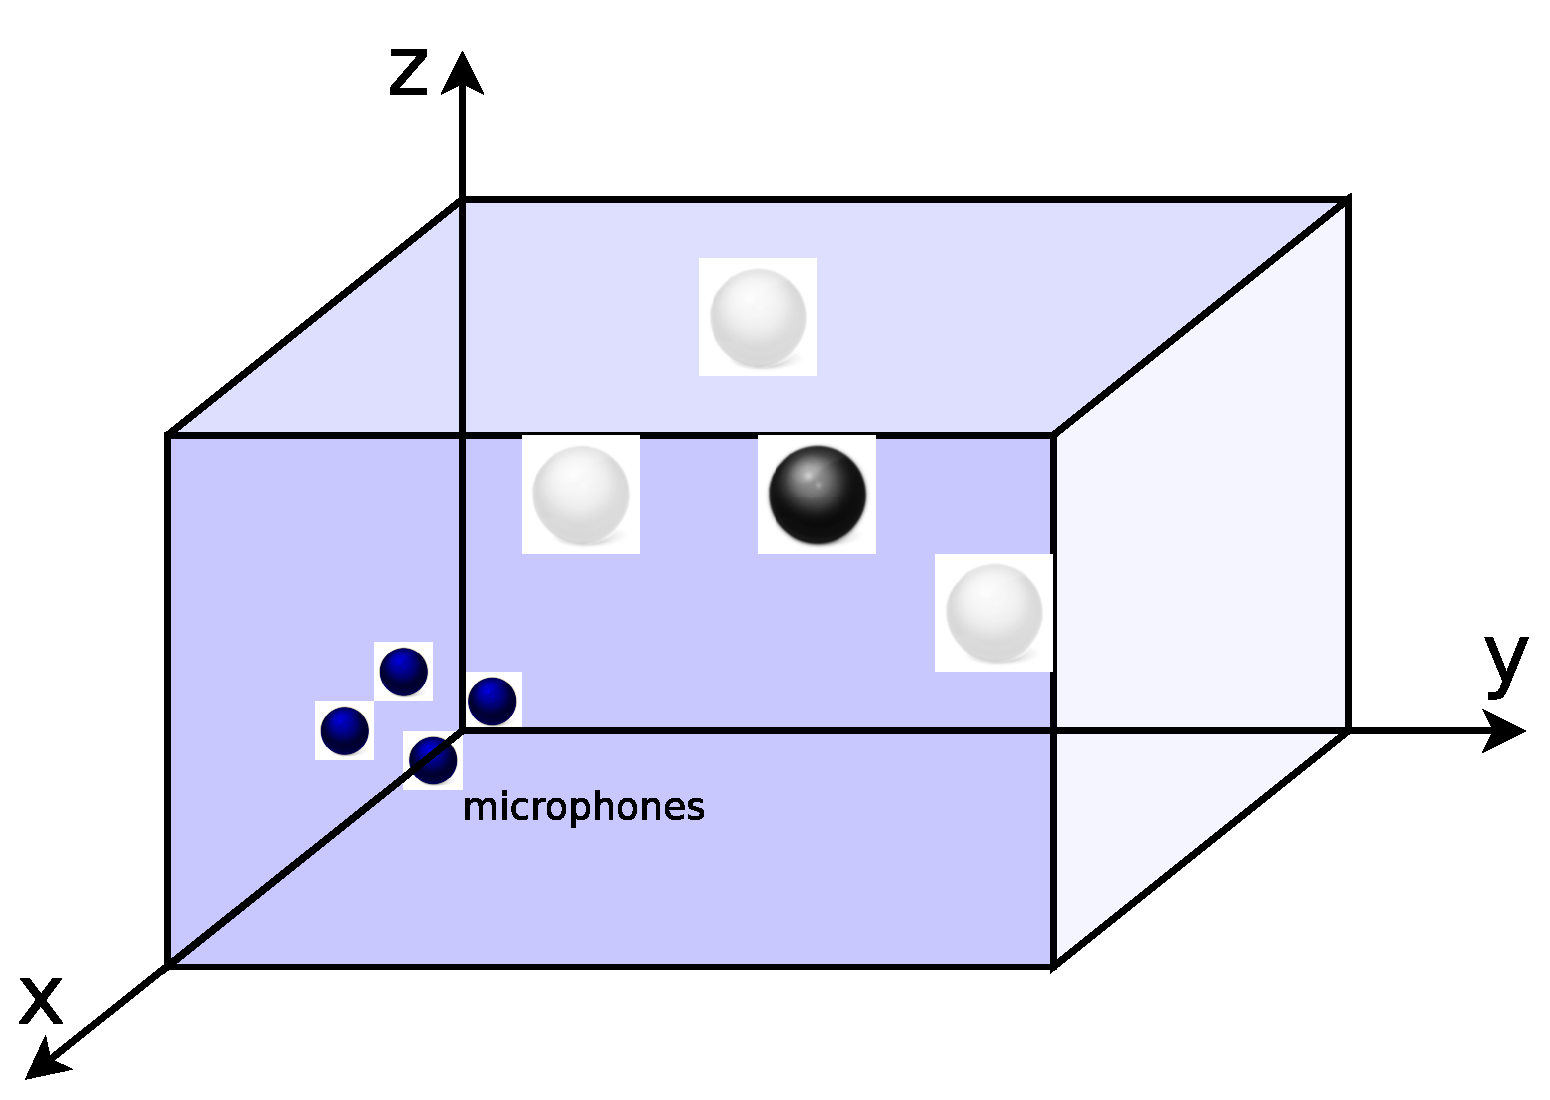
\includegraphics[width=70mm]{room_diagram.eps}} \\
  \subfloat[\label{fig:image_method}] {
    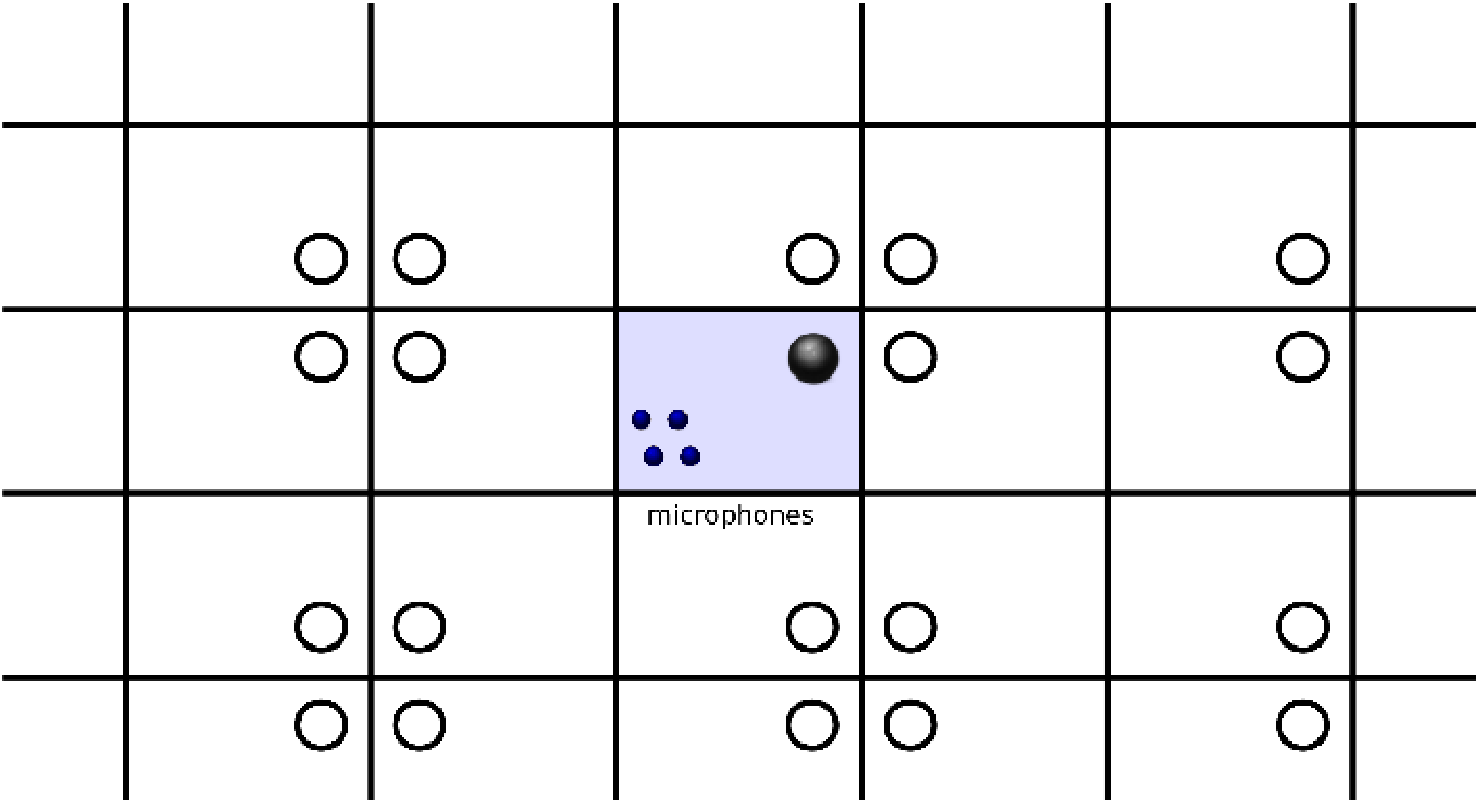
\includegraphics[width=70mm]{image_method.eps}}
   \caption{
    (a) A simulated room: There may be multiple microphones, a single target
    sound source, multiple noise sources in a cuboid-shape room with
    acoustically reflective walls. (b) A diagram showing the location
    of the real and the virtual sound sources assuming that the walls
    reflects acoustic wave like a mirror \cite{C_Kim_INTERSPEECH_2017_1}.}
  \end{center}
  \vspace{-10mm}
\end{figure}
%
%
In this section, we briefly review the structure of the Google
Room Simulator for generating simulated utterances
to train acoustic models for speech recognition systems
\cite{C_Kim_INTERSPEECH_2017_1}. We assume a room of a
rectangular cuboid-shape as shown in Fig. \ref{fig:room_diagram}.
Assuming that all the walls of a room reflect acoustically uniformly,
we use the image method to model the Room Impulse Responses (RIRs)
\cite{J_Allen_JASA_1979, E_A_Lehmann_ASPAA_2007, S_G_McGovern_RIR}.

Fig. \ref{fig:image_method} shows how virtual sources
appearing as empty circles are constructed in the image method.
Even though the virtual rooms appear to be created in two-dimensions
in Fig. \ref{fig:image_method}, in the ``\emph{Room Simulator}",
they are constructed in three-dimensions. For example, in our
work for training the acoustic model for Google Home, we consider
$17 \times 17 \times 17 = 4913$ virtual rooms for RIR calculation
\cite{C_Kim_INTERSPEECH_2017_1}.
Following the image method, the impulse response is calculated
using the following equation
\cite{ J_Allen_JASA_1979, E_A_Lehmann_ASPAA_2007}:
\begin{align}
    h[n] = \sum_{i = 0}^{I-1} \frac{r^{g_i}}{d_i}
    \delta \left[n -\left \lceil{\frac{d_i f_s}{c_0}}\right \rceil \right],
      \label{eq:h_n_calculation}
\end{align}
where $i$ is the index of each virtual sound source, and $d_i$ is the distance
from that sound source to the microphone, $r$ is
the reflection coefficient of the wall, $g_i$ is
the number of the reflections
to that sound source, $f_s$ is the sampling rate of the RIR, and $c_0$ is the
speed of sound in the air. We use the value of $f_s = 16,000$ \textit{Hz} and
$c_0 = 343$ \textit{m/s} for the room simulator \cite{B_Li_INTERSPEECH_2017_1}.
For $d_i$, $r$, we use numbers created by a random number generator
following specified distributions for each impulse response \cite{C_Kim_INTERSPEECH_2017_1}.

Assuming that there are $I$ sound sources including one target
source and $J$ microphones, the received signal at microphone
$j$ is given by:
\begin{align}
  y_j[n] =  \sum_{i=0}^{I-1} \alpha_{ij} \left(h_{ij}[n] * x_i[n]\right).
  \label{eq:y_j_def}
\end{align}
Since we used a two-microphones system in
\cite{B_Li_INTERSPEECH_2017_1, C_Kim_INTERSPEECH_2017_1},
$J$ is two, and for the number noise sources, we used a value from zero
up to three \cite{C_Kim_INTERSPEECH_2017_1}.
%
%
%
%
%
%
%\begin{figure}[!tbp]
%  \begin{center}
%    \resizebox{75mm}{!}{% Graphic for TeX using PGF
% Title: /google/src/cloud/chanwcom/chanwcom-speech9999/google3/experimental/users/chanwcom/my_papers/papers_working/icml_2018_feature_mapping_spl/figures/entire_diagram.dia
% Creator: Dia v0.97.2
% CreationDate: Fri Nov 24 23:29:46 2017
% For: chanwcom
% \usepackage{tikz}
% The following commands are not supported in PSTricks at present
% We define them conditionally, so when they are implemented,
% this pgf file will use them.
\ifx\du\undefined
  \newlength{\du}
\fi
\setlength{\du}{15\unitlength}
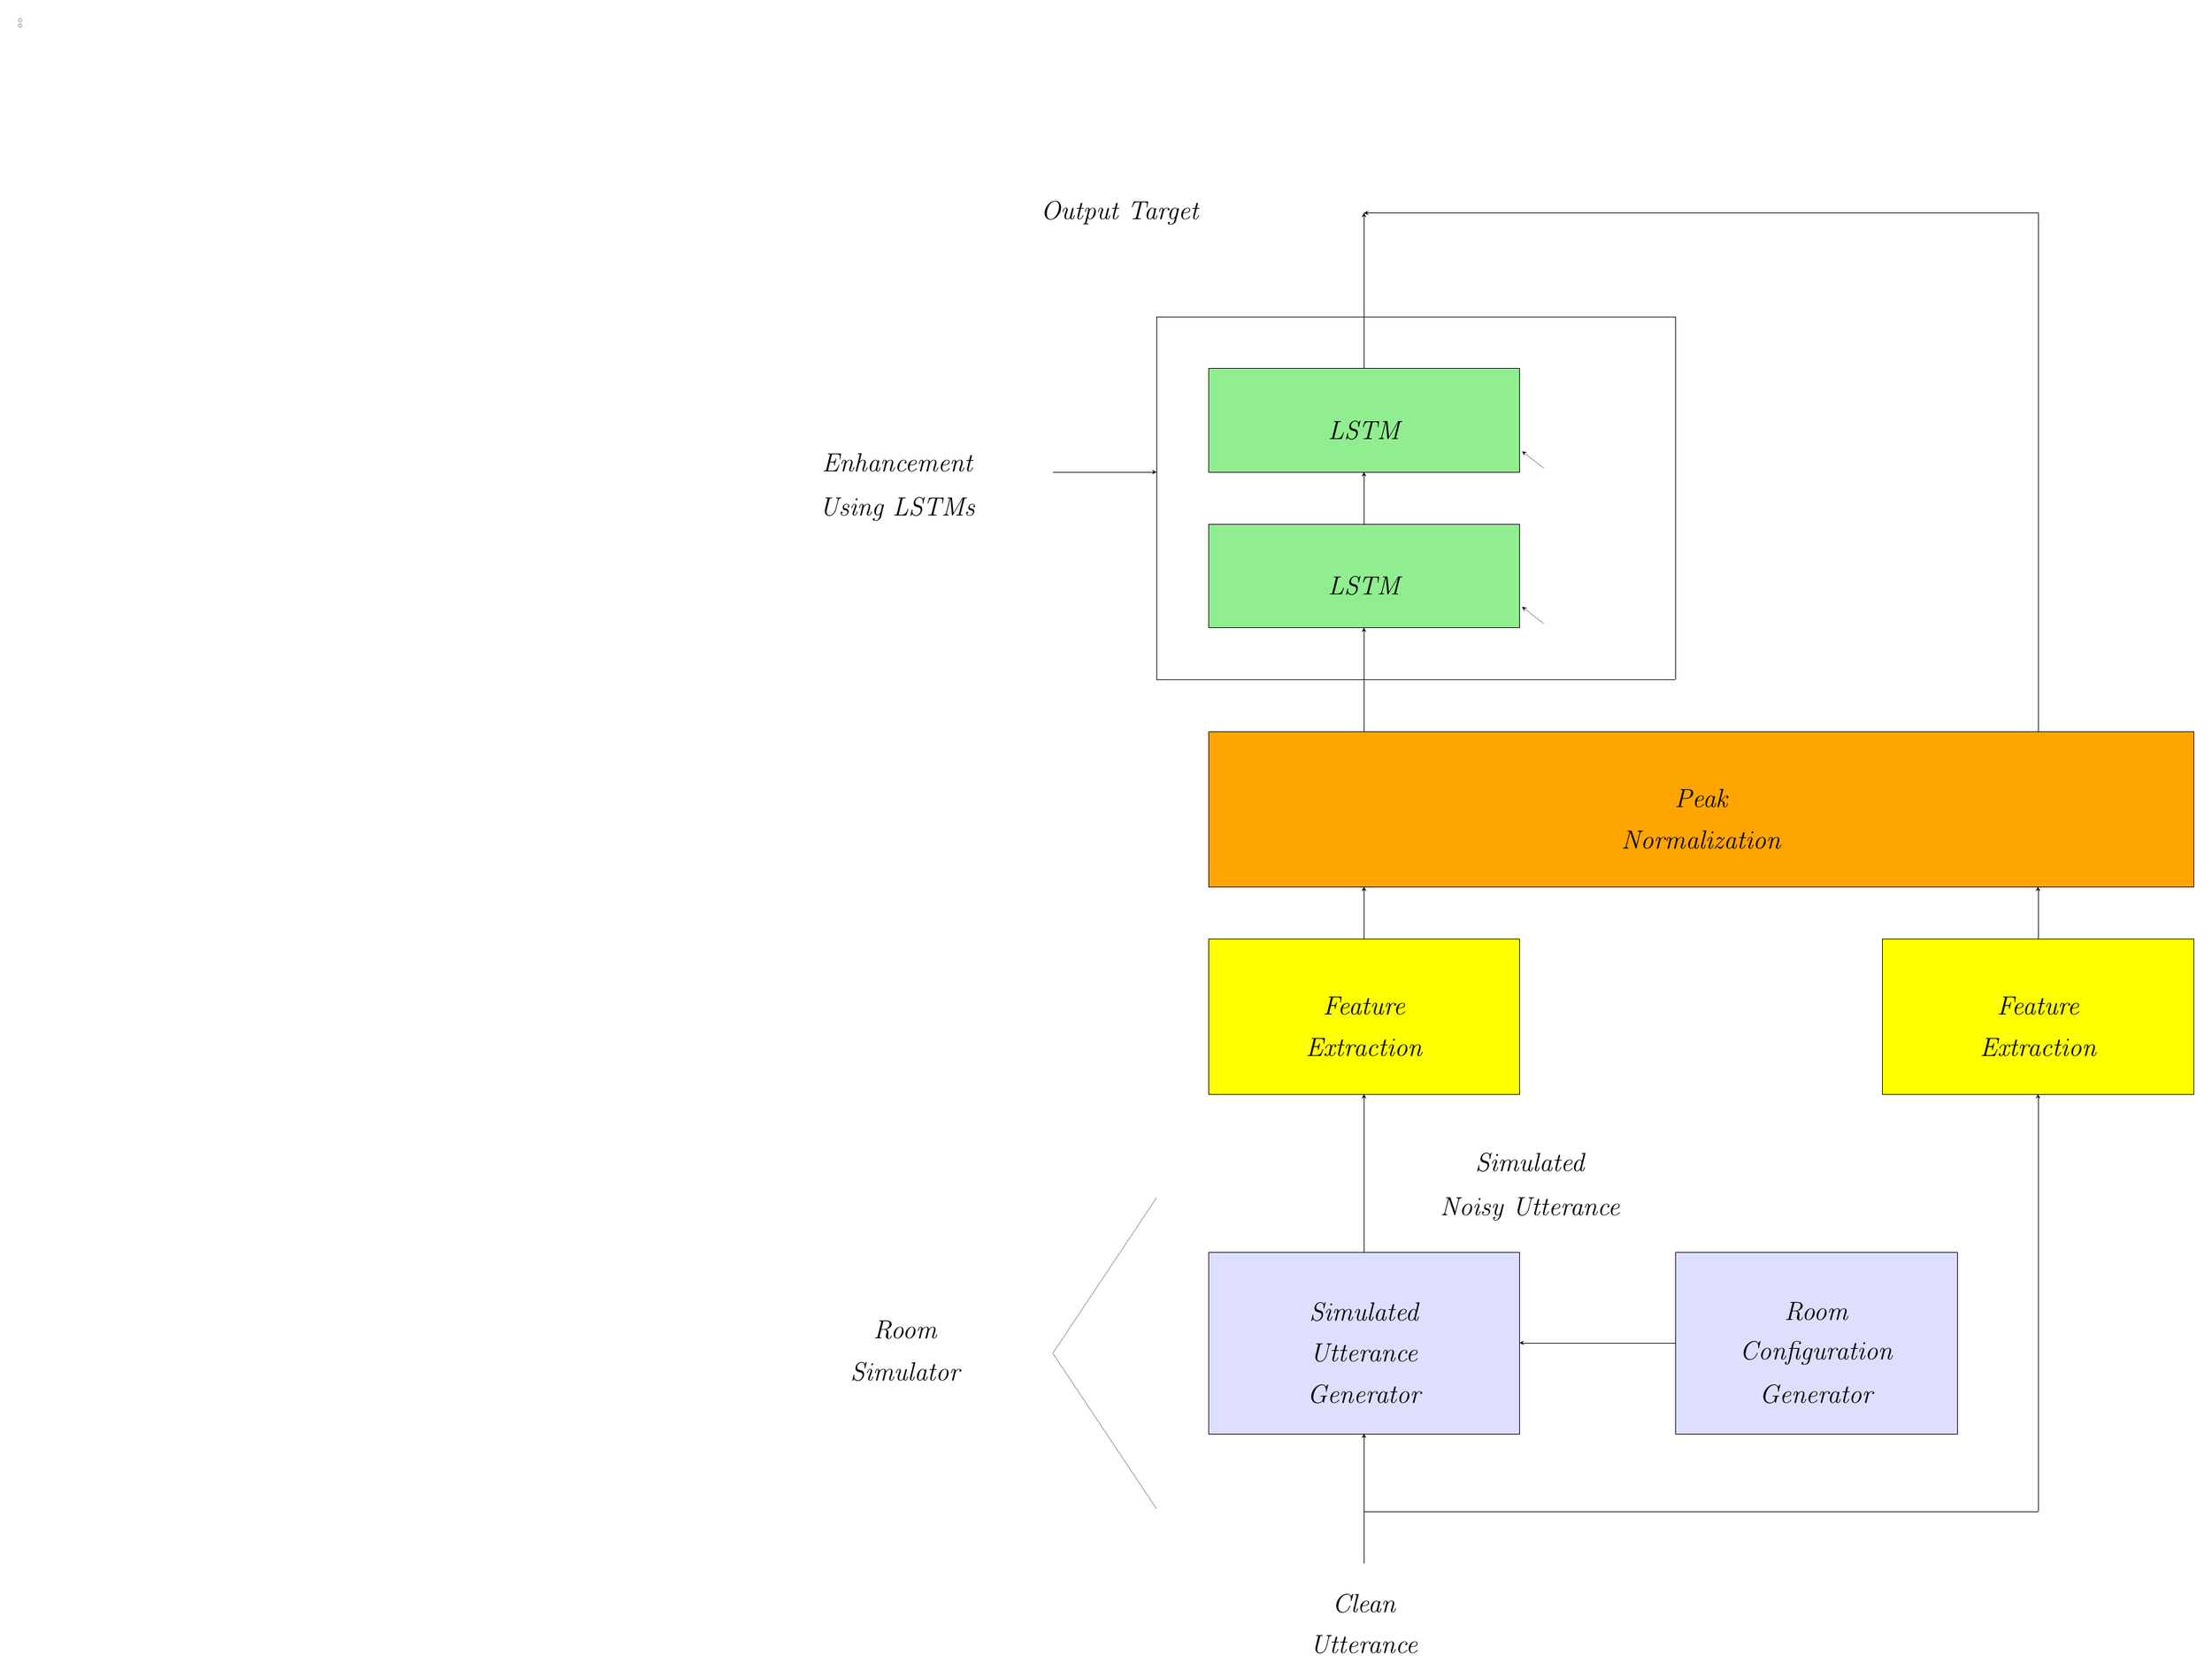
\begin{tikzpicture}
  \tikzstyle{every node}=[font=\Large\itshape]
\pgftransformxscale{1.000000}
\pgftransformyscale{-1.000000}
\definecolor{dialinecolor}{rgb}{0.000000, 0.000000, 0.000000}
\pgfsetstrokecolor{dialinecolor}
\definecolor{dialinecolor}{rgb}{1.000000, 1.000000, 1.000000}
\pgfsetfillcolor{dialinecolor}
\definecolor{dialinecolor}{rgb}{1.000000, 1.000000, 1.000000}
\pgfsetfillcolor{dialinecolor}
\fill (23.000000\du,6.000000\du)--(23.000000\du,13.000000\du)--(33.000000\du,13.000000\du)--(33.000000\du,6.000000\du)--cycle;
\pgfsetlinewidth{0.100000\du}
\pgfsetdash{{\pgflinewidth}{0.200000\du}}{0cm}
\pgfsetdash{{\pgflinewidth}{0.200000\du}}{0cm}
\pgfsetmiterjoin
\definecolor{dialinecolor}{rgb}{0.000000, 0.000000, 0.000000}
\pgfsetstrokecolor{dialinecolor}
\draw (23.000000\du,6.000000\du)--(23.000000\du,13.000000\du)--(33.000000\du,13.000000\du)--(33.000000\du,6.000000\du)--cycle;
% setfont left to latex
\definecolor{dialinecolor}{rgb}{0.000000, 0.000000, 0.000000}
\pgfsetstrokecolor{dialinecolor}
\node at (28.000000\du,9.695000\du){};
\definecolor{dialinecolor}{rgb}{0.870588, 0.870588, 1.000000}
\pgfsetfillcolor{dialinecolor}
\fill (24.000000\du,24.050000\du)--(24.000000\du,27.550000\du)--(30.000000\du,27.550000\du)--(30.000000\du,24.050000\du)--cycle;
\pgfsetlinewidth{0.100000\du}
\pgfsetdash{}{0pt}
\pgfsetdash{}{0pt}
\pgfsetmiterjoin
\definecolor{dialinecolor}{rgb}{0.000000, 0.000000, 0.000000}
\pgfsetstrokecolor{dialinecolor}
\draw (24.000000\du,24.050000\du)--(24.000000\du,27.550000\du)--(30.000000\du,27.550000\du)--(30.000000\du,24.050000\du)--cycle;
% setfont left to latex
\definecolor{dialinecolor}{rgb}{0.000000, 0.000000, 0.000000}
\pgfsetstrokecolor{dialinecolor}
\node at (27.000000\du,25.195000\du){Simulated};
% setfont left to latex
\definecolor{dialinecolor}{rgb}{0.000000, 0.000000, 0.000000}
\pgfsetstrokecolor{dialinecolor}
\node at (27.000000\du,25.995000\du){Utterance};
% setfont left to latex
\definecolor{dialinecolor}{rgb}{0.000000, 0.000000, 0.000000}
\pgfsetstrokecolor{dialinecolor}
\node at (27.000000\du,26.795000\du){Generator};
% setfont left to latex
\definecolor{dialinecolor}{rgb}{0.000000, 0.000000, 0.000000}
\pgfsetstrokecolor{dialinecolor}
\node[anchor=west] at (27.000000\du,25.800000\du){};
\pgfsetlinewidth{0.100000\du}
\pgfsetdash{}{0pt}
\pgfsetdash{}{0pt}
\pgfsetbuttcap
{
\definecolor{dialinecolor}{rgb}{0.000000, 0.000000, 0.000000}
\pgfsetfillcolor{dialinecolor}
% was here!!!
\pgfsetarrowsend{stealth}
\definecolor{dialinecolor}{rgb}{0.000000, 0.000000, 0.000000}
\pgfsetstrokecolor{dialinecolor}
\draw (40.000000\du,29.050000\du)--(40.000000\du,21.000000\du);
}
\pgfsetlinewidth{0.100000\du}
\pgfsetdash{}{0pt}
\pgfsetdash{}{0pt}
\pgfsetbuttcap
{
\definecolor{dialinecolor}{rgb}{0.000000, 0.000000, 0.000000}
\pgfsetfillcolor{dialinecolor}
% was here!!!
\pgfsetarrowsend{stealth}
\definecolor{dialinecolor}{rgb}{0.000000, 0.000000, 0.000000}
\pgfsetstrokecolor{dialinecolor}
\draw (27.000000\du,24.050000\du)--(27.000000\du,21.000000\du);
}
\definecolor{dialinecolor}{rgb}{1.000000, 1.000000, 1.000000}
\pgfsetfillcolor{dialinecolor}
\pgfpathellipse{\pgfpoint{30.850000\du}{11.000000\du}}{\pgfpoint{1.000000\du}{0\du}}{\pgfpoint{0\du}{1.000000\du}}
\pgfusepath{fill}
\pgfsetlinewidth{0.100000\du}
\pgfsetdash{}{0pt}
\pgfsetdash{}{0pt}
\pgfsetmiterjoin
\definecolor{dialinecolor}{rgb}{0.000000, 0.000000, 0.000000}
\pgfsetstrokecolor{dialinecolor}
\pgfpathellipse{\pgfpoint{30.850000\du}{11.000000\du}}{\pgfpoint{1.000000\du}{0\du}}{\pgfpoint{0\du}{1.000000\du}}
\pgfusepath{stroke}
% setfont left to latex
\definecolor{dialinecolor}{rgb}{0.000000, 0.000000, 0.000000}
\pgfsetstrokecolor{dialinecolor}
\node at (30.850000\du,11.195000\du){};
\pgfsetlinewidth{0.100000\du}
\pgfsetdash{}{0pt}
\pgfsetdash{}{0pt}
\pgfsetbuttcap
{
\definecolor{dialinecolor}{rgb}{0.000000, 0.000000, 0.000000}
\pgfsetfillcolor{dialinecolor}
% was here!!!
\pgfsetarrowsend{stealth}
\definecolor{dialinecolor}{rgb}{0.000000, 0.000000, 0.000000}
\pgfsetstrokecolor{dialinecolor}
\draw (30.467300\du,11.923900\du)--(30.050000\du,11.600000\du);
}
\definecolor{dialinecolor}{rgb}{1.000000, 1.000000, 1.000000}
\pgfsetfillcolor{dialinecolor}
\pgfpathellipse{\pgfpoint{30.850000\du}{8.000000\du}}{\pgfpoint{1.000000\du}{0\du}}{\pgfpoint{0\du}{1.000000\du}}
\pgfusepath{fill}
\pgfsetlinewidth{0.100000\du}
\pgfsetdash{}{0pt}
\pgfsetdash{}{0pt}
\pgfsetmiterjoin
\definecolor{dialinecolor}{rgb}{0.000000, 0.000000, 0.000000}
\pgfsetstrokecolor{dialinecolor}
\pgfpathellipse{\pgfpoint{30.850000\du}{8.000000\du}}{\pgfpoint{1.000000\du}{0\du}}{\pgfpoint{0\du}{1.000000\du}}
\pgfusepath{stroke}
% setfont left to latex
\definecolor{dialinecolor}{rgb}{0.000000, 0.000000, 0.000000}
\pgfsetstrokecolor{dialinecolor}
\node at (30.850000\du,8.195000\du){};
\pgfsetlinewidth{0.100000\du}
\pgfsetdash{}{0pt}
\pgfsetdash{}{0pt}
\pgfsetbuttcap
{
\definecolor{dialinecolor}{rgb}{0.000000, 0.000000, 0.000000}
\pgfsetfillcolor{dialinecolor}
% was here!!!
\pgfsetarrowsend{stealth}
\definecolor{dialinecolor}{rgb}{0.000000, 0.000000, 0.000000}
\pgfsetstrokecolor{dialinecolor}
\draw (30.467300\du,8.923880\du)--(30.050000\du,8.600000\du);
}
\definecolor{dialinecolor}{rgb}{0.564706, 0.933333, 0.564706}
\pgfsetfillcolor{dialinecolor}
\fill (24.000000\du,7.000000\du)--(24.000000\du,9.000000\du)--(30.000000\du,9.000000\du)--(30.000000\du,7.000000\du)--cycle;
\pgfsetlinewidth{0.100000\du}
\pgfsetdash{}{0pt}
\pgfsetdash{}{0pt}
\pgfsetmiterjoin
\definecolor{dialinecolor}{rgb}{0.000000, 0.000000, 0.000000}
\pgfsetstrokecolor{dialinecolor}
\draw (24.000000\du,7.000000\du)--(24.000000\du,9.000000\du)--(30.000000\du,9.000000\du)--(30.000000\du,7.000000\du)--cycle;
% setfont left to latex
\definecolor{dialinecolor}{rgb}{0.000000, 0.000000, 0.000000}
\pgfsetstrokecolor{dialinecolor}
\node at (27.000000\du,8.195000\du){LSTM};
\definecolor{dialinecolor}{rgb}{0.564706, 0.933333, 0.564706}
\pgfsetfillcolor{dialinecolor}
\fill (24.000000\du,10.000000\du)--(24.000000\du,12.000000\du)--(30.000000\du,12.000000\du)--(30.000000\du,10.000000\du)--cycle;
\pgfsetlinewidth{0.100000\du}
\pgfsetdash{}{0pt}
\pgfsetdash{}{0pt}
\pgfsetmiterjoin
\definecolor{dialinecolor}{rgb}{0.000000, 0.000000, 0.000000}
\pgfsetstrokecolor{dialinecolor}
\draw (24.000000\du,10.000000\du)--(24.000000\du,12.000000\du)--(30.000000\du,12.000000\du)--(30.000000\du,10.000000\du)--cycle;
% setfont left to latex
\definecolor{dialinecolor}{rgb}{0.000000, 0.000000, 0.000000}
\pgfsetstrokecolor{dialinecolor}
\node at (27.000000\du,11.195000\du){LSTM};
\pgfsetlinewidth{0.100000\du}
\pgfsetdash{}{0pt}
\pgfsetdash{}{0pt}
\pgfsetbuttcap
{
\definecolor{dialinecolor}{rgb}{0.000000, 0.000000, 0.000000}
\pgfsetfillcolor{dialinecolor}
% was here!!!
\pgfsetarrowsend{stealth}
\definecolor{dialinecolor}{rgb}{0.000000, 0.000000, 0.000000}
\pgfsetstrokecolor{dialinecolor}
\draw (27.000000\du,14.000000\du)--(27.000000\du,12.000000\du);
}
\pgfsetlinewidth{0.100000\du}
\pgfsetdash{}{0pt}
\pgfsetdash{}{0pt}
\pgfsetbuttcap
{
\definecolor{dialinecolor}{rgb}{0.000000, 0.000000, 0.000000}
\pgfsetfillcolor{dialinecolor}
% was here!!!
\pgfsetarrowsend{stealth}
\definecolor{dialinecolor}{rgb}{0.000000, 0.000000, 0.000000}
\pgfsetstrokecolor{dialinecolor}
\draw (27.000000\du,10.000000\du)--(27.000000\du,9.000000\du);
}
\pgfsetlinewidth{0.100000\du}
\pgfsetdash{}{0pt}
\pgfsetdash{}{0pt}
\pgfsetbuttcap
{
\definecolor{dialinecolor}{rgb}{0.000000, 0.000000, 0.000000}
\pgfsetfillcolor{dialinecolor}
% was here!!!
\definecolor{dialinecolor}{rgb}{0.000000, 0.000000, 0.000000}
\pgfsetstrokecolor{dialinecolor}
\draw (40.000000\du,14.000000\du)--(40.000000\du,4.000000\du);
}
% setfont left to latex
\definecolor{dialinecolor}{rgb}{0.000000, 0.000000, 0.000000}
\pgfsetstrokecolor{dialinecolor}
\node[anchor=west] at (20.650000\du,4.000000\du){Output Target};
\definecolor{dialinecolor}{rgb}{0.870588, 0.870588, 1.000000}
\pgfsetfillcolor{dialinecolor}
\fill (33.000000\du,24.050000\du)--(33.000000\du,27.550000\du)--(38.440000\du,27.550000\du)--(38.440000\du,24.050000\du)--cycle;
\pgfsetlinewidth{0.100000\du}
\pgfsetdash{}{0pt}
\pgfsetdash{}{0pt}
\pgfsetmiterjoin
\definecolor{dialinecolor}{rgb}{0.000000, 0.000000, 0.000000}
\pgfsetstrokecolor{dialinecolor}
\draw (33.000000\du,24.050000\du)--(33.000000\du,27.550000\du)--(38.440000\du,27.550000\du)--(38.440000\du,24.050000\du)--cycle;
% setfont left to latex
\definecolor{dialinecolor}{rgb}{0.000000, 0.000000, 0.000000}
\pgfsetstrokecolor{dialinecolor}
\node at (35.720000\du,25.195000\du){Room};
% setfont left to latex
\definecolor{dialinecolor}{rgb}{0.000000, 0.000000, 0.000000}
\pgfsetstrokecolor{dialinecolor}
\node at (35.720000\du,25.995000\du){Configuration};
% setfont left to latex
\definecolor{dialinecolor}{rgb}{0.000000, 0.000000, 0.000000}
\pgfsetstrokecolor{dialinecolor}
\node at (35.720000\du,26.795000\du){Generator};
\pgfsetlinewidth{0.100000\du}
\pgfsetdash{}{0pt}
\pgfsetdash{}{0pt}
\pgfsetbuttcap
{
\definecolor{dialinecolor}{rgb}{0.000000, 0.000000, 0.000000}
\pgfsetfillcolor{dialinecolor}
% was here!!!
\pgfsetarrowsend{stealth}
\definecolor{dialinecolor}{rgb}{0.000000, 0.000000, 0.000000}
\pgfsetstrokecolor{dialinecolor}
\draw (33.000000\du,25.800000\du)--(30.000000\du,25.800000\du);
}
\definecolor{dialinecolor}{rgb}{1.000000, 1.000000, 0.000000}
\pgfsetfillcolor{dialinecolor}
\fill (37.000000\du,18.000000\du)--(37.000000\du,21.000000\du)--(43.000000\du,21.000000\du)--(43.000000\du,18.000000\du)--cycle;
\pgfsetlinewidth{0.100000\du}
\pgfsetdash{}{0pt}
\pgfsetdash{}{0pt}
\pgfsetmiterjoin
\definecolor{dialinecolor}{rgb}{0.000000, 0.000000, 0.000000}
\pgfsetstrokecolor{dialinecolor}
\draw (37.000000\du,18.000000\du)--(37.000000\du,21.000000\du)--(43.000000\du,21.000000\du)--(43.000000\du,18.000000\du)--cycle;
% setfont left to latex
\definecolor{dialinecolor}{rgb}{0.000000, 0.000000, 0.000000}
\pgfsetstrokecolor{dialinecolor}
\node at (40.000000\du,19.295000\du){Feature};
% setfont left to latex
\definecolor{dialinecolor}{rgb}{0.000000, 0.000000, 0.000000}
\pgfsetstrokecolor{dialinecolor}
\node at (40.000000\du,20.095000\du){Extraction};
\pgfsetlinewidth{0.100000\du}
\pgfsetdash{}{0pt}
\pgfsetdash{}{0pt}
\pgfsetbuttcap
{
\definecolor{dialinecolor}{rgb}{0.000000, 0.000000, 0.000000}
\pgfsetfillcolor{dialinecolor}
% was here!!!
\definecolor{dialinecolor}{rgb}{0.000000, 0.000000, 0.000000}
\pgfsetstrokecolor{dialinecolor}
\draw (27.000000\du,29.050000\du)--(40.000000\du,29.050000\du);
}
\definecolor{dialinecolor}{rgb}{1.000000, 1.000000, 0.000000}
\pgfsetfillcolor{dialinecolor}
\fill (24.000000\du,18.000000\du)--(24.000000\du,21.000000\du)--(30.000000\du,21.000000\du)--(30.000000\du,18.000000\du)--cycle;
\pgfsetlinewidth{0.100000\du}
\pgfsetdash{}{0pt}
\pgfsetdash{}{0pt}
\pgfsetmiterjoin
\definecolor{dialinecolor}{rgb}{0.000000, 0.000000, 0.000000}
\pgfsetstrokecolor{dialinecolor}
\draw (24.000000\du,18.000000\du)--(24.000000\du,21.000000\du)--(30.000000\du,21.000000\du)--(30.000000\du,18.000000\du)--cycle;
% setfont left to latex
\definecolor{dialinecolor}{rgb}{0.000000, 0.000000, 0.000000}
\pgfsetstrokecolor{dialinecolor}
\node at (27.000000\du,19.295000\du){Feature};
% setfont left to latex
\definecolor{dialinecolor}{rgb}{0.000000, 0.000000, 0.000000}
\pgfsetstrokecolor{dialinecolor}
\node at (27.000000\du,20.095000\du){Extraction};
\pgfsetlinewidth{0.100000\du}
\pgfsetdash{}{0pt}
\pgfsetdash{}{0pt}
\pgfsetbuttcap
{
\definecolor{dialinecolor}{rgb}{0.000000, 0.000000, 0.000000}
\pgfsetfillcolor{dialinecolor}
% was here!!!
\pgfsetarrowsend{stealth}
\definecolor{dialinecolor}{rgb}{0.000000, 0.000000, 0.000000}
\pgfsetstrokecolor{dialinecolor}
\draw (40.000000\du,18.000000\du)--(40.000000\du,17.000000\du);
}
\definecolor{dialinecolor}{rgb}{1.000000, 0.647059, 0.000000}
\pgfsetfillcolor{dialinecolor}
\fill (24.000000\du,14.000000\du)--(24.000000\du,17.000000\du)--(43.000000\du,17.000000\du)--(43.000000\du,14.000000\du)--cycle;
\pgfsetlinewidth{0.100000\du}
\pgfsetdash{}{0pt}
\pgfsetdash{}{0pt}
\pgfsetmiterjoin
\definecolor{dialinecolor}{rgb}{0.000000, 0.000000, 0.000000}
\pgfsetstrokecolor{dialinecolor}
\draw (24.000000\du,14.000000\du)--(24.000000\du,17.000000\du)--(43.000000\du,17.000000\du)--(43.000000\du,14.000000\du)--cycle;
% setfont left to latex
\definecolor{dialinecolor}{rgb}{0.000000, 0.000000, 0.000000}
\pgfsetstrokecolor{dialinecolor}
\node at (33.500000\du,15.295000\du){Peak};
% setfont left to latex
\definecolor{dialinecolor}{rgb}{0.000000, 0.000000, 0.000000}
\pgfsetstrokecolor{dialinecolor}
\node at (33.500000\du,16.095000\du){Normalization};
\pgfsetlinewidth{0.100000\du}
\pgfsetdash{}{0pt}
\pgfsetdash{}{0pt}
\pgfsetbuttcap
{
\definecolor{dialinecolor}{rgb}{0.000000, 0.000000, 0.000000}
\pgfsetfillcolor{dialinecolor}
% was here!!!
\pgfsetarrowsend{stealth}
\definecolor{dialinecolor}{rgb}{0.000000, 0.000000, 0.000000}
\pgfsetstrokecolor{dialinecolor}
\draw (27.000000\du,18.000000\du)--(27.000000\du,17.000000\du);
}
\pgfsetlinewidth{0.100000\du}
\pgfsetdash{}{0pt}
\pgfsetdash{}{0pt}
\pgfsetbuttcap
{
\definecolor{dialinecolor}{rgb}{0.000000, 0.000000, 0.000000}
\pgfsetfillcolor{dialinecolor}
% was here!!!
\pgfsetarrowsend{stealth}
\definecolor{dialinecolor}{rgb}{0.000000, 0.000000, 0.000000}
\pgfsetstrokecolor{dialinecolor}
\draw (27.000000\du,30.050000\du)--(27.000000\du,27.550000\du);
}
\pgfsetlinewidth{0.100000\du}
\pgfsetdash{}{0pt}
\pgfsetdash{}{0pt}
\pgfsetbuttcap
{
\definecolor{dialinecolor}{rgb}{0.000000, 0.000000, 0.000000}
\pgfsetfillcolor{dialinecolor}
% was here!!!
\pgfsetarrowsend{stealth}
\definecolor{dialinecolor}{rgb}{0.000000, 0.000000, 0.000000}
\pgfsetstrokecolor{dialinecolor}
\draw (40.000000\du,4.000000\du)--(27.000000\du,4.000000\du);
}
\pgfsetlinewidth{0.100000\du}
\pgfsetdash{}{0pt}
\pgfsetdash{}{0pt}
\pgfsetbuttcap
{
\definecolor{dialinecolor}{rgb}{0.000000, 0.000000, 0.000000}
\pgfsetfillcolor{dialinecolor}
% was here!!!
\pgfsetarrowsend{stealth}
\definecolor{dialinecolor}{rgb}{0.000000, 0.000000, 0.000000}
\pgfsetstrokecolor{dialinecolor}
\draw (27.000000\du,7.000000\du)--(27.000000\du,4.000000\du);
}
\pgfsetlinewidth{0.100000\du}
\pgfsetdash{}{0pt}
\pgfsetdash{}{0pt}
\pgfsetbuttcap
{
\definecolor{dialinecolor}{rgb}{0.000000, 0.000000, 0.000000}
\pgfsetfillcolor{dialinecolor}
% was here!!!
\definecolor{dialinecolor}{rgb}{0.000000, 0.000000, 0.000000}
\pgfsetstrokecolor{dialinecolor}
\draw (23.000000\du,23.000000\du)--(21.000000\du,26.000000\du);
}
\pgfsetlinewidth{0.100000\du}
\pgfsetdash{}{0pt}
\pgfsetdash{}{0pt}
\pgfsetbuttcap
{
\definecolor{dialinecolor}{rgb}{0.000000, 0.000000, 0.000000}
\pgfsetfillcolor{dialinecolor}
% was here!!!
\definecolor{dialinecolor}{rgb}{0.000000, 0.000000, 0.000000}
\pgfsetstrokecolor{dialinecolor}
\draw (23.000000\du,29.000000\du)--(21.000000\du,26.000000\du);
}
% setfont left to latex
\definecolor{dialinecolor}{rgb}{0.000000, 0.000000, 0.000000}
\pgfsetstrokecolor{dialinecolor}
\node at (18.150000\du,25.550000\du){Room};
% setfont left to latex
\definecolor{dialinecolor}{rgb}{0.000000, 0.000000, 0.000000}
\pgfsetstrokecolor{dialinecolor}
\node at (18.150000\du,26.350000\du){Simulator};
\pgfsetlinewidth{0.100000\du}
\pgfsetdash{}{0pt}
\pgfsetdash{}{0pt}
\pgfsetbuttcap
{
\definecolor{dialinecolor}{rgb}{0.000000, 0.000000, 0.000000}
\pgfsetfillcolor{dialinecolor}
% was here!!!
\pgfsetarrowsend{stealth}
\definecolor{dialinecolor}{rgb}{0.000000, 0.000000, 0.000000}
\pgfsetstrokecolor{dialinecolor}
\draw (21.000000\du,9.000000\du)--(23.000000\du,9.000000\du);
}
% setfont left to latex
\definecolor{dialinecolor}{rgb}{0.000000, 0.000000, 0.000000}
\pgfsetstrokecolor{dialinecolor}
\node at (18.000000\du,8.821250\du){Enhancement};
% setfont left to latex
\definecolor{dialinecolor}{rgb}{0.000000, 0.000000, 0.000000}
\pgfsetstrokecolor{dialinecolor}
\node at (18.000000\du,9.721250\du){Using LSTMs};
% setfont left to latex
\definecolor{dialinecolor}{rgb}{0.000000, 0.000000, 0.000000}
\pgfsetstrokecolor{dialinecolor}
\node at (27.000000\du,30.821250\du){Clean};
% setfont left to latex
\definecolor{dialinecolor}{rgb}{0.000000, 0.000000, 0.000000}
\pgfsetstrokecolor{dialinecolor}
\node at (27.000000\du,31.621250\du){Utterance};
% setfont left to latex
\definecolor{dialinecolor}{rgb}{0.000000, 0.000000, 0.000000}
\pgfsetstrokecolor{dialinecolor}
\node at (30.200000\du,22.321250\du){Simulated};
% setfont left to latex
\definecolor{dialinecolor}{rgb}{0.000000, 0.000000, 0.000000}
\pgfsetstrokecolor{dialinecolor}
\node at (30.200000\du,23.221250\du){Noisy Utterance};
\end{tikzpicture}
}
%      \caption {
%        The architecture for acoustic model training using
%        the room simulator and LSTMs and a DNN (LDNN)
%     \cite{T_Sainath_ICASSP_2016_1, C_Kim_INTERSPEECH_2017_1}. }
%          \label{fig:entire_diagram}
%  \end{center}
%\vspace{-7mm}
%\end{figure}
%
%
%
%%
%\begin{figure}%[tbp]
%  \begin{center}
%    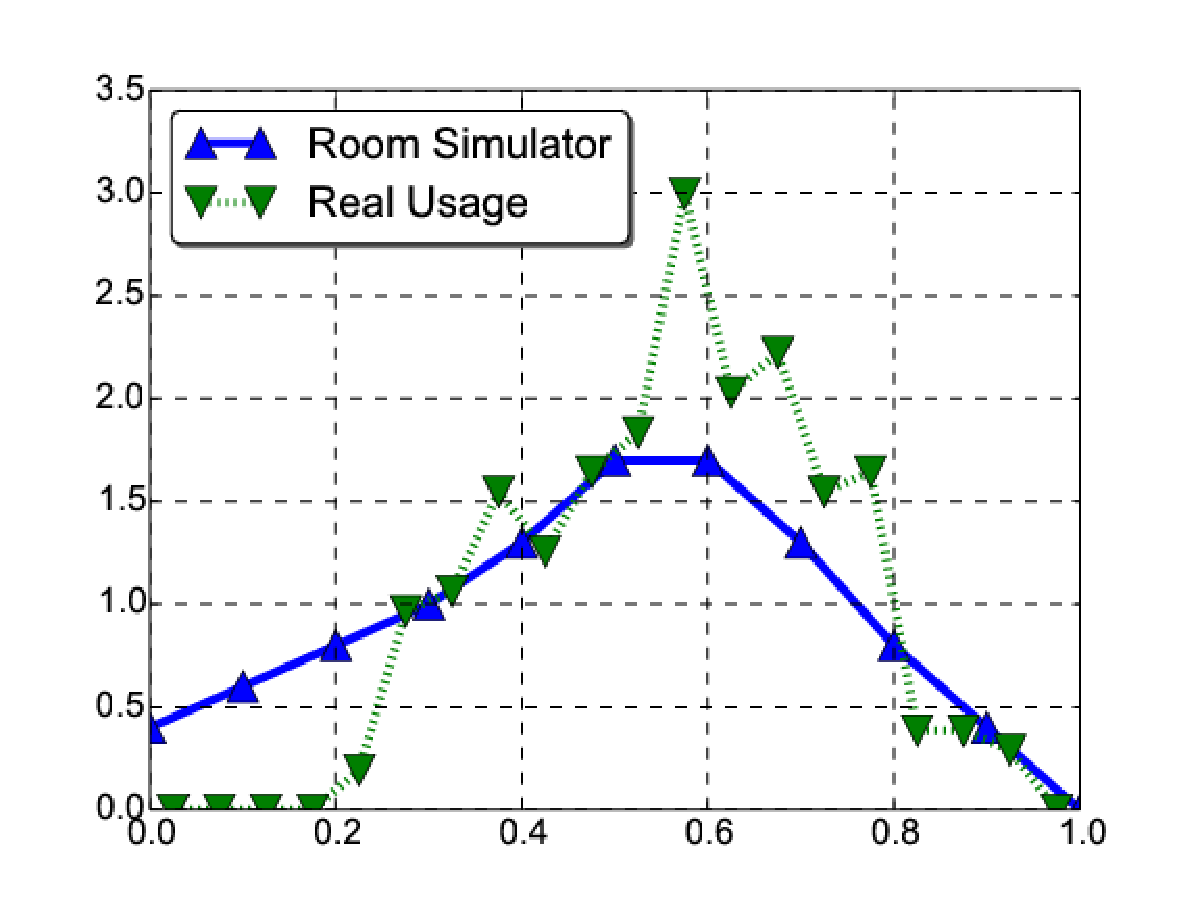
\includegraphics[width=70mm]{reverb_time_distribution}
%    \label{fig:target_length}
%    \caption {
%      Reverberation time ($T_{60}$) distribution in our
%      configuration for training the acoustic model for Google Home
%      and the real Google Home user usage.
%    }
%   \vspace{-7mm}
%  \end{center}
%\end{figure}
%

%
%
%
\subsection{Efficient Room Impulse Response filtering}
%
%
%
When the signal and the room impulse response length are $N_x$ and
$M$, respectively, to calculate \eqref{eq:y_j_def} using the time-domain
convolution, the number of multiplications $C_{td}$ is given by:
\begin{align}
  C_{td} = I \times J \times  M  \times N_x.
  \label{eq:num_mults_linear_convolution}
\end{align}
In our training set used in Sec. \ref{sec:experimental_results},
the average utterance length including \emph{non-speech} portions
marked by the Voice Activity Detector (VAD) is 6.35 \textit{s}.
This corresponds to $N_x$ of 101,523 at 16 \textit{kHz}. The average
length of the RIR in the room simulator used in
\cite{C_Kim_INTERSPEECH_2017_1} is 0.243 \textit{s} \AR{Sounds a bit too smalle?}, corresponding
to the $M$ value of 3893.
For Google Home the number of noise sources in our training
set is 1.55 on average.
Thus $I$ is 1.55 including one target source, and $J$ is two, since
we use a two-microphones system in
\cite{C_Kim_INTERSPEECH_2017_1, B_Li_INTERSPEECH_2017_1}.
Thus, if we directly use the linear convolution, it requires
two billion multiplications per utterance from
\eqref{eq:num_mults_linear_convolution}, which is prohibitively large.
Thus, in the ``\textit{Room Simulator}" in
\cite{C_Kim_INTERSPEECH_2017_1},
we used the frequency domain multiplication using \texttt{Kiss FFT}
\cite{M_Borgerding_kiss_fft_2010}. To avoid time aliasing,
the FFT size $N$ must satisfy $N \ge N_x + M - 1$.
The $j$-th microphone channel
of the simulated signal $y_j[n]$ in \eqref{eq:y_j_def}
\begin{align}
  y_{j} [n] = \sum_{i=0}^{I-1}FFT^{-1} \left \{
      FFT \left \{ h_{ij}[n] \right \} \times
      FFT \left \{ x_i[n] \right \}
      \right \}  %* FFT\{X_i[omega_k}\}\}
\end{align}
Considering we perform two FFTs \AR{Why 2? You should consider speech and 1.55 noises right?}, one IFFT, and one complex spectrum
element-wise multiplications, the number of real multiplications
$C_{\textit{FFT}}$ is given by:
\begin{align}
  C_{\textit{FFT}} = 6 N \log_2(N) + 4 N.
  \label{eq:c_fft}
\end{align}
where $N$ is the FFT size. \AR{Shouldn't all this be in big-O notation? So not exactly NlogN but O(NlogN)?} The number of real multiplications
in \eqref{eq:c_fft} is based on the assumption that a single FFT 
requires $\frac{N}{2} \log_2(N)$ multiplications \AR{This is confusing, I think it makes sense to just use NlogN given you are already ignoring other constants that are not O(NlogN).}, and a single
complex multiplication requires four real multiplications. The $4N$
term in \eqref{eq:c_fft} appears since there is one frequency domain
element-wise multiplications.
If we use $N = 2 ^ {17}$, it requires 70.9 million multiplications
per utterance. The room simulator was implemented in C++ using
the \texttt{Eigen3} linear algebra library \cite{eigenweb}.
In \texttt{Eigen3}, \texttt{Kiss FFT} \cite{M_Borgerding_kiss_fft_2010} and \texttt{FFTW3}
\cite{M_Frigo_proceedings_of_the_ieee_20015} are unofficially supported.
We used the \texttt{Kiss FFT} version of FFT in \texttt{Eigen3} since
there were some technical issues in using \texttt{FFTW3} in \texttt{Eigen3}
to run on \texttt{Google Borg} cluster \cite{A_Verma_eurosys_2015_1}.
But, to fruther speed up frontend computation, we switched from
\texttt{Kiss FFT} in \texttt{Eigen3} to a custom  C++ class
implementation which internally using real FFT in \texttt{FFTW3}.
\AR{The argument seems weak. Consider rephrasing? Maybe say, our initial implementation was based on KissFFT. But, to further speed up computation, we switched ... i.e., don't mention about technical issues on borg cluster -- that seems something very specific and scientifically uninteresting.}

A more efficient approach is using the OverLap Add (OLA)
FFT filtering \AR{cite?}. With the OLA FFT filtering,
the approximate number of real multiplications is given by:
\begin{align}
  C_{\textit{OLA}} =  \left \lfloor{\frac{N_x}{N - M + 1}}\right \rfloor
  \left[4 N \log_2(N) + 4 N  \right] + 2 N \log_2(N)
  \label{eq:c_ola}
\end{align}
where $N$ is the FFT size, $N_x$ is the length of the entire
signal, and $M$ is the length of the impulse response. The term
$4 N \log_2(N) + 4 N $ appears in \eqref{eq:c_ola}, since there is
one FFT and one IFFT for each block. 
$\left \lfloor{\frac{N_x}{N - M + 1}}\right \rfloor$
is the number of blocks to process an utterance of length $N_x$.
The $2 N \log_2(N)$ term in \eqref{eq:c_ola} is the required multiplications
for the impulse response. For the impulse response $h_{ij}[n]$, we do not
need to repeat it for every block.
In our training set consisting of 22 million utterances, the
average utterance length is 7.31 \textit{s} \AR{Earlier you said it is 6.55s, Fix?}.
Then we can find we find the optimal value of $M = 11300$, and the
number of approximate number of real multiplication is 39.2 millions.
%
%
%
%
\subsection{Room Impulse Response Length Selection}
%
%In our original implementation of the room simulator, we covered up to
%17 reflections. The RIR length depends on the room size we used in the
%simulator. Since we used a distribution of room size, the RIR length is
%not fixed.
%Even though the reverberation time is usually given in terms of
%$T_{60}$, which is defined to be the time for XXX.
%
The average length of the Room Impulse Response in the original room
simulator is estimated to be 3893 samples, which corresponds to 0.243
\textit{s}.
%
We perform a simple RIR tail-cutoff by finding the RIR power threshold
which is $\eta$ \textit{dB} below the maximum power of the RIR
$h_{ij}[n]$:
\begin{align}
  p_{th} = \max \left \{h_{ij}^2[n] \right \} \times 10^{-\frac{\eta}{10}}.
\end{align}
Using $p_{th}$, we find the cut-off index $n_c$ which is the smallest
sample index beyond which all the trailing $h_{ij}[n]$ has power
below the threshold $p_{th}$:
\begin{align}
  n_c = \min_{m} \left\{
  m \middle| \max_{n > m} \left\{  h^2[n] \right \} <  p_{th}  \right \}.
\end{align}
Then the final RIR cut-off $\widehat{h}_{ij}[n]$ is given
by the following equation:
\begin{align}
  \widehat{h}_{ij}[n] = h_{ij}[n], \qquad 0 \le n \le n_c + 1.
\end{align}
Fig. \ref{fig:rir_cutoff} shows impulse responses when different RIR
cutoff threshold $\eta$ is used. To reflect the typical case in
our training set, we used the average room dimension, average
microphone-to-target distance, and average $T_{60}$ value among
3 million room configurations described in \cite{C_Kim_INTERSPEECH_2017_1}.

As shown in Table \ref{tbl:local_machine_prof} and \ref{tbl:cpu_percentage},
the RIR tail cut-off at 20 \textit{dB} shows relatively 35.6 \% to 69.4 \%
speed improvement on a local desktop machine and on \texttt{Google Borg}
cluster \cite{A_Verma_eurosys_2015_1}.
Fig. \ref{fig:rir_cutoff_local_profiling} shows the profiling results
on a local machine with different RIR cutoff thresholds $\eta$.
The local machine we used has a single \texttt{Intel(R) Xeon(R) CPU E5-1650 @ 3.20GHz}
CPU with 6 cores and 32 GB of memory. In Fig. \ref{fig:rir_cutoff_local_profiling},
we observe that the computational cost becomes less for the OLA filtering
case as we cut the tail portion of the RIR more. For the full FFT case,
theoretically, it should remain almost constant regardless of the
impulse response length, but due to variation
in profiling measurement, there is some small variation.
%
%\begin{figure}%[tbp]
%  \begin{center}
%    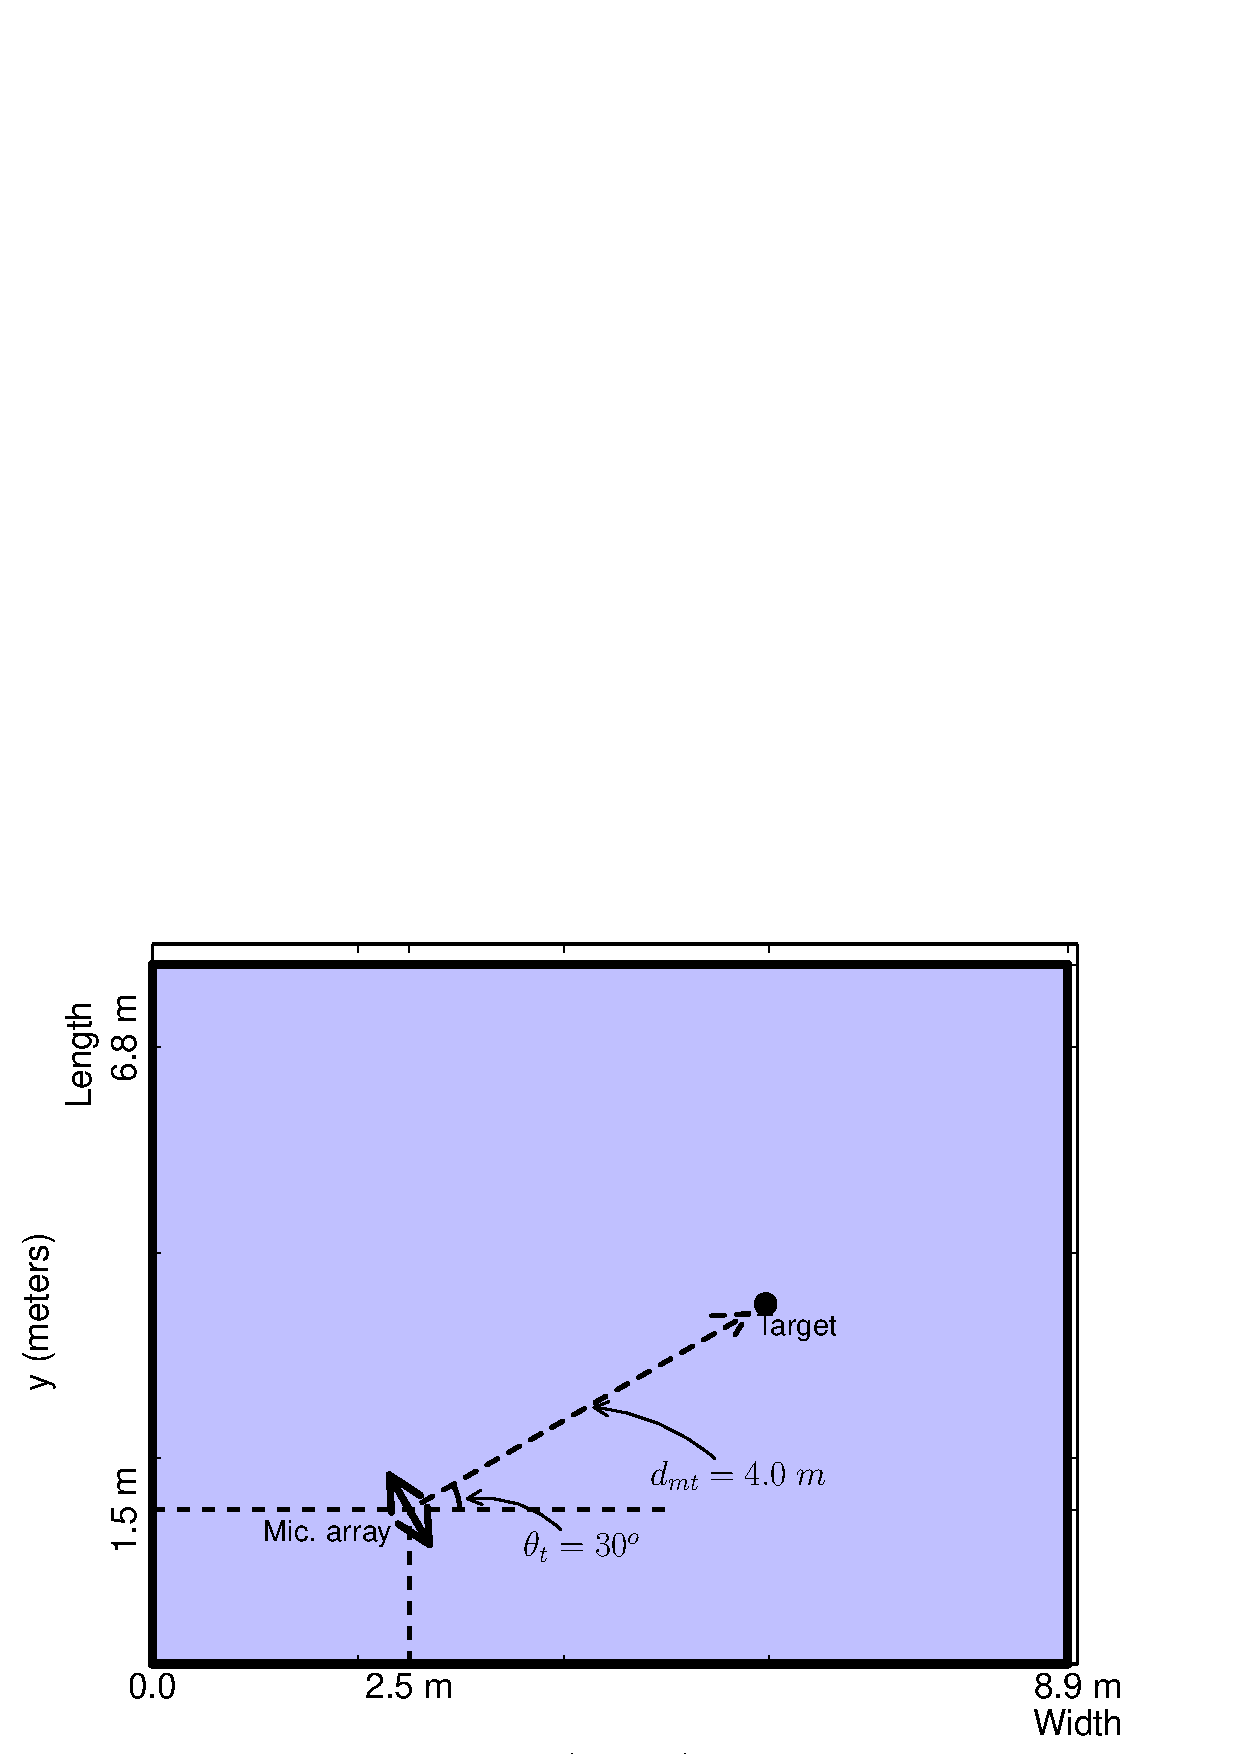
\includegraphics[width=70mm]{plot_mic_source_target_2d_asymmetric}
%      \caption { Room configuration used for generating Room Impulse Responses (RIRs)
%         in Fig. \ref{fig:rir_cutoff}
%      \ref{sec:experimental_results}}
%          \label{fig:room_configuration}
%    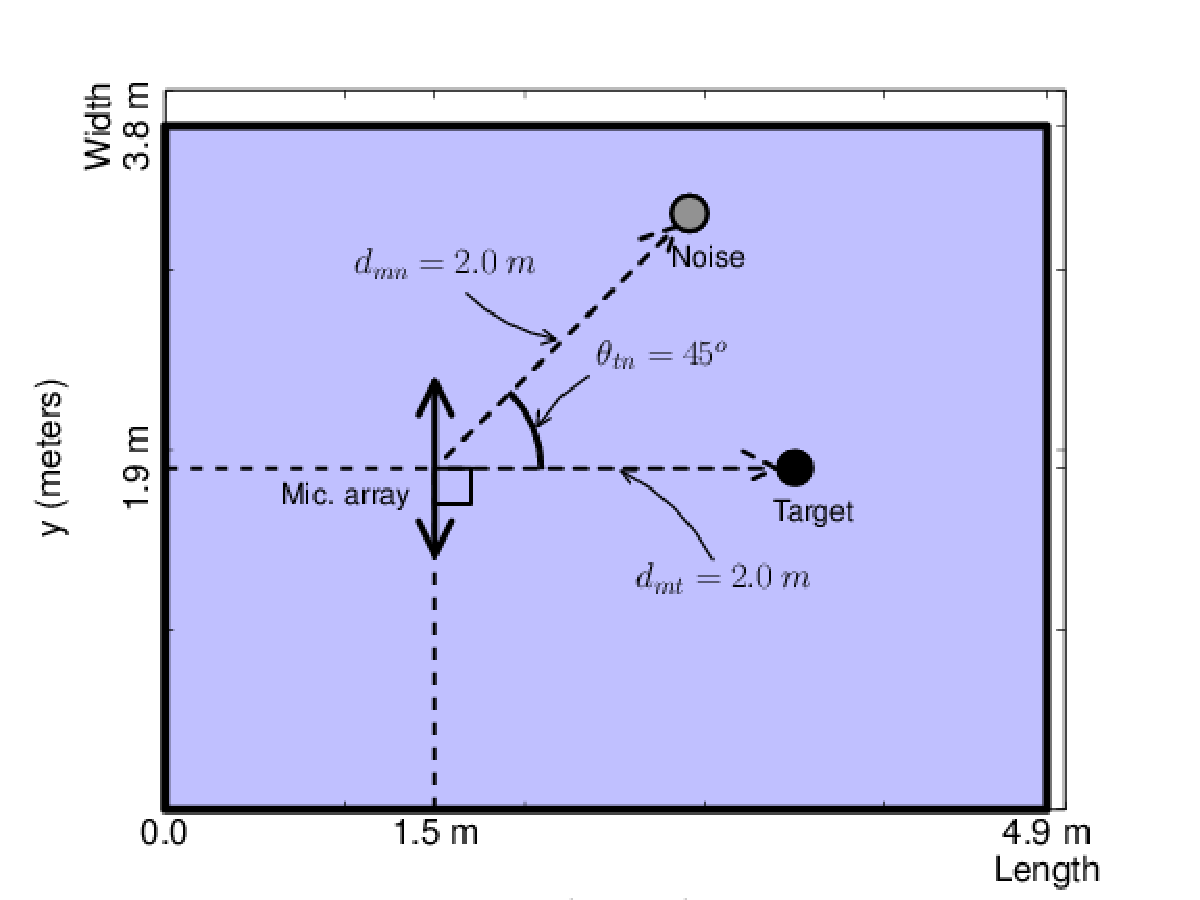
\includegraphics[width=50mm]{plot_mic_source_target_2d_symmetric}
%      \caption { A microphone array with two microphones in an anechoic chamber.
%      The azimuth angle with respect to the $x$-axis is $\theta$. }
%          \label{fig:recording_room_final}
%  \vspace{-7mm}
%  \end{center}
%\end{figure}
%
%\begin{figure}[tbp]
%  \begin{center}
%    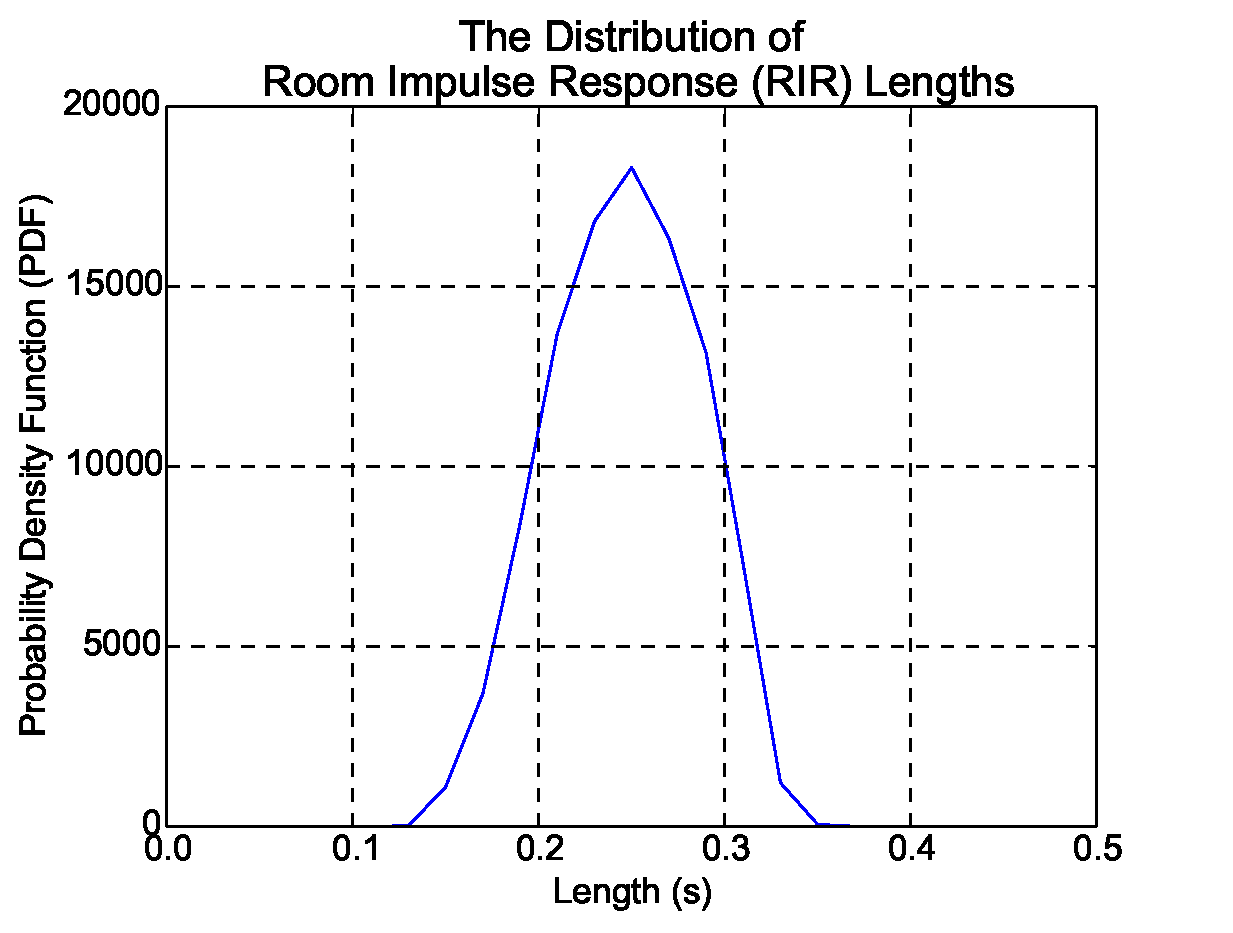
\includegraphics[width=70mm]{target_length}
%    \label{fig:target_length}
%    \caption {
%      Word Error Rates (WERs) for the voice search test set 
%      at different reverberation time corrupted by (a) an
%      interfering speaker and (b) various noise in the 
%      DEMAND noise database.
%    }   
%   \vspace{-7mm}
%  \end{center}
%\end{figure}
%
\begin{figure}%[tbp]
  \begin{center}
    \subfloat[] {
      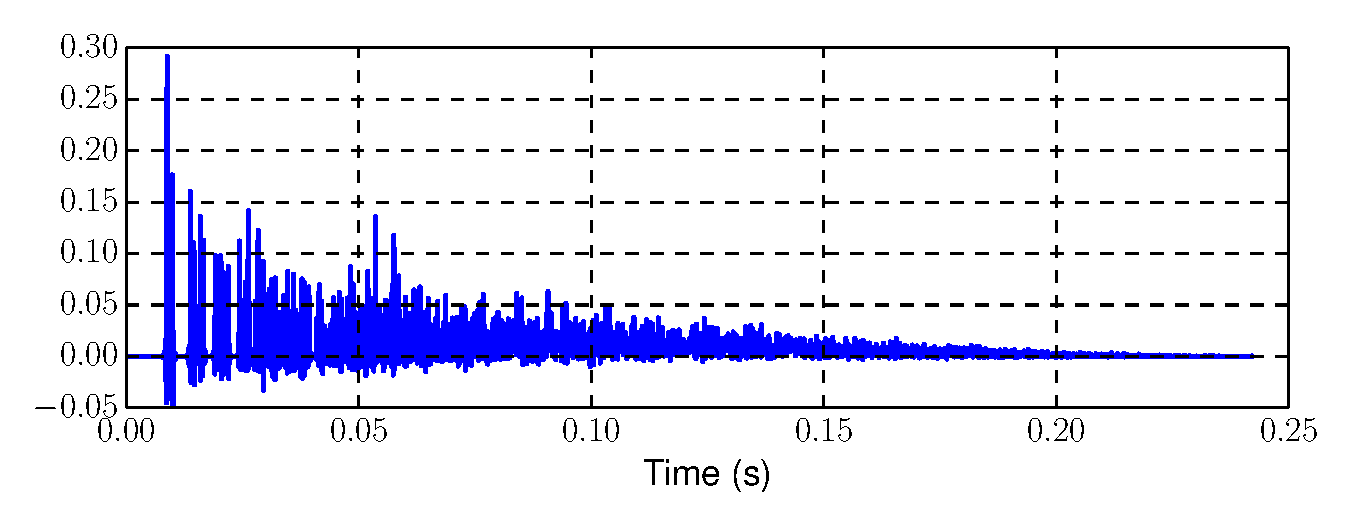
\includegraphics[width=70mm]{rir_no_cutoff}
      \label{fig:rir_cutoff_simulated_sets}
    }
    \vspace{-5mm}
    \\
    \subfloat[] {
      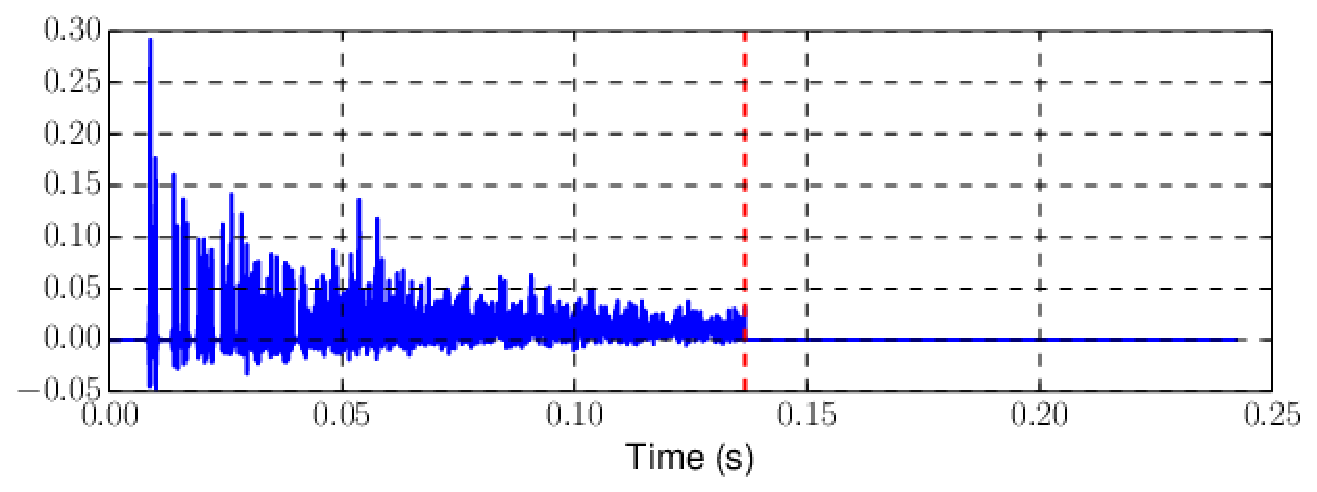
\includegraphics[width=70mm]{rir_20db_cutoff}
      \label{fig:rir_cutoff_rerecorded_sets}
    }
    \vspace{-5mm}
    \\
%    \subfloat[] {
%      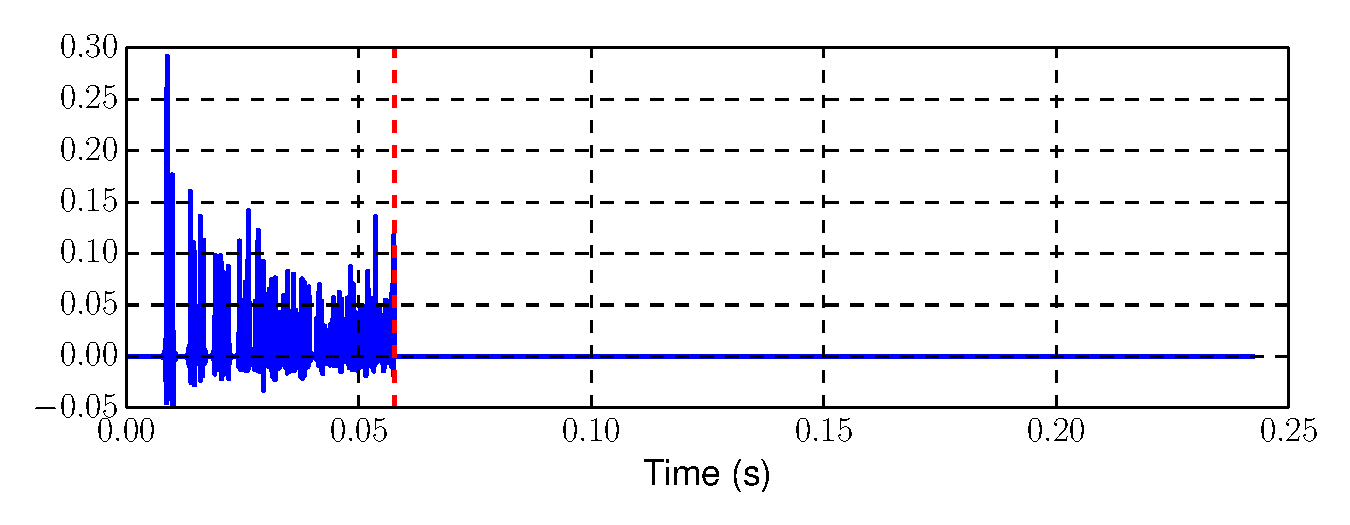
\includegraphics[width=70mm]{rir_10db_cutoff}
%      \label{fig:rir_cutoff_rerecorded_sets}
%    }
%    \\
    \subfloat[] {
      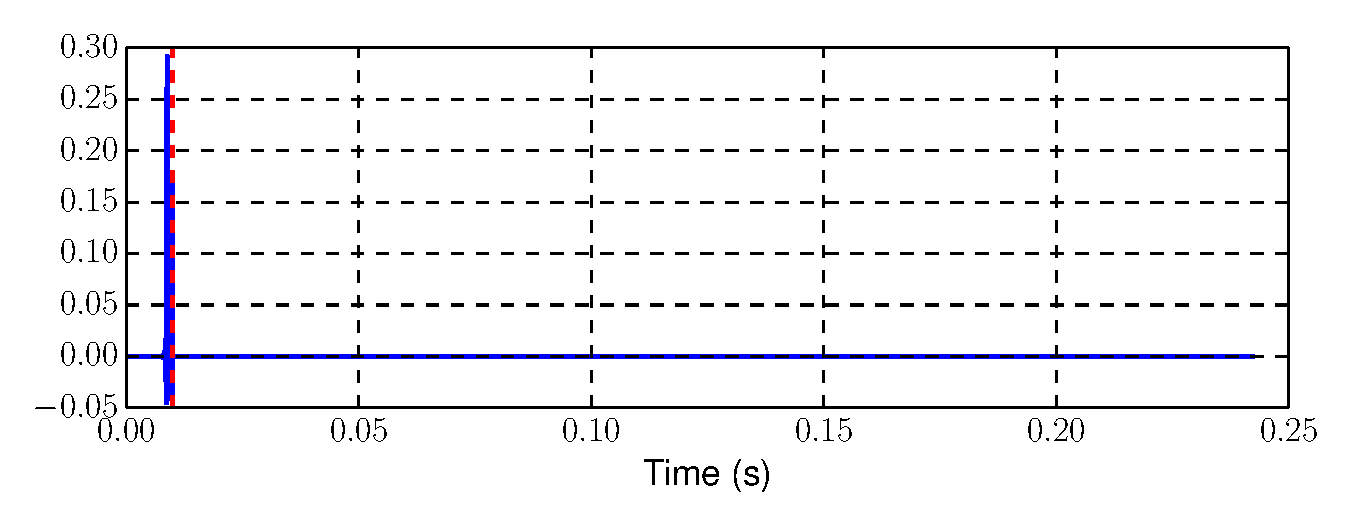
\includegraphics[width=70mm]{rir_5db_cutoff}
      \label{fig:rir_cutoff_rerecorded_sets}
    }
    \caption {
      The simulated room impulse responses generated in the
      ``Room Simulator" described in Sec. \ref{sec:implementation}:
      (a) The impulse response without the RIR tail cut-off,
      (b) with the RIR tail cut-off at 20 \textit{dB},
      and (c) with the RIR tail cut-off at 5 \textit{dB}.
    }
   \vspace{-7mm}
  \label{fig:rir_cutoff}
  \end{center}
\end{figure}
%
%
%\begin{figure}%[tbp]
%  \begin{center}
%    \subfloat[] {
%      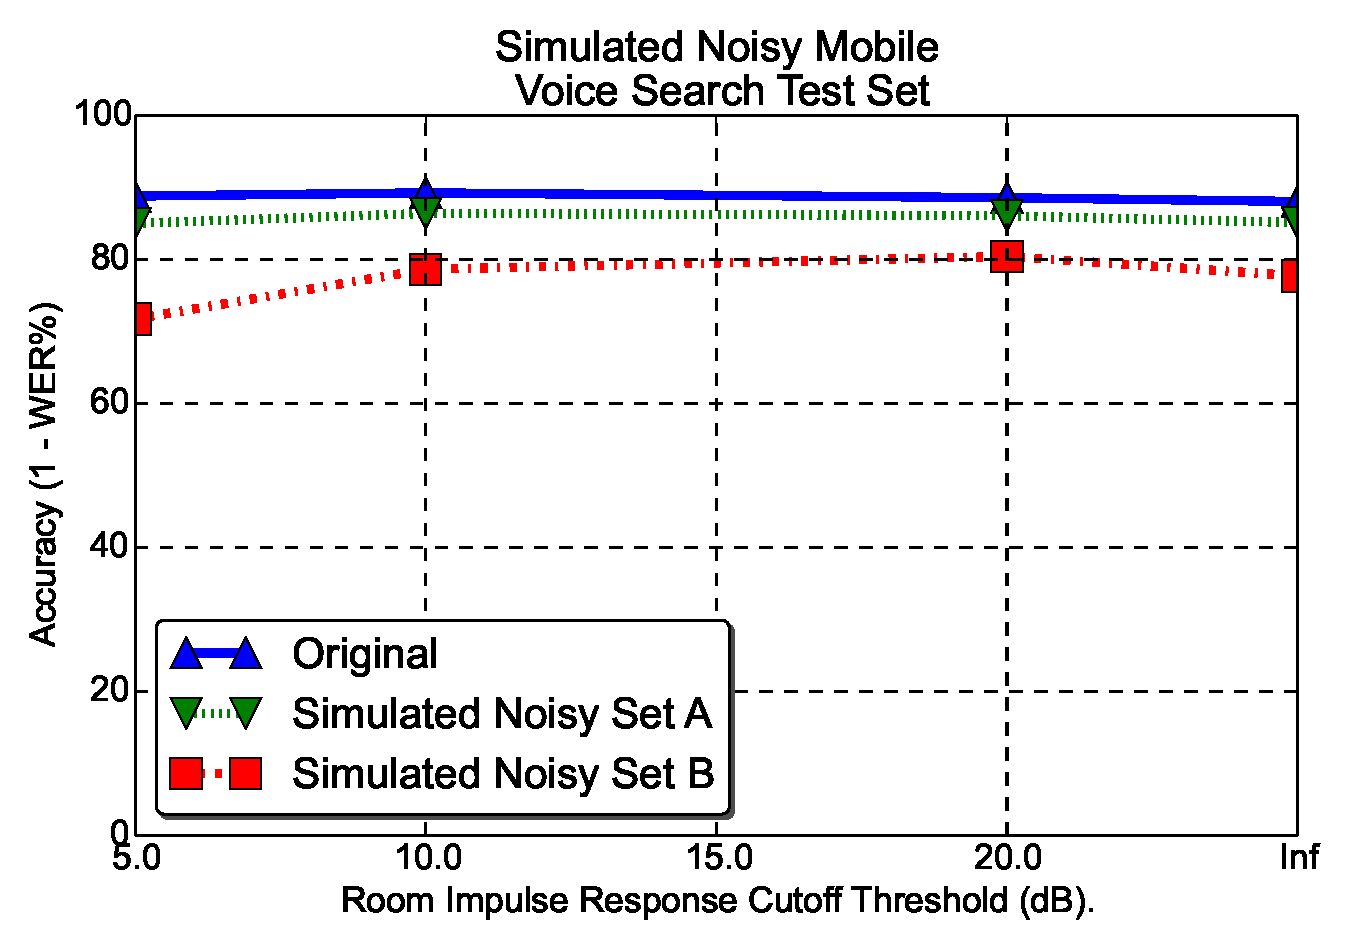
\includegraphics[width=70mm]{rir_cutoff_simulated_sets}
%      \label{fig:rir_cutoff_simulated_sets}
%    }
%    \vspace{-4mm}
%    \\
%    \subfloat[] {
%      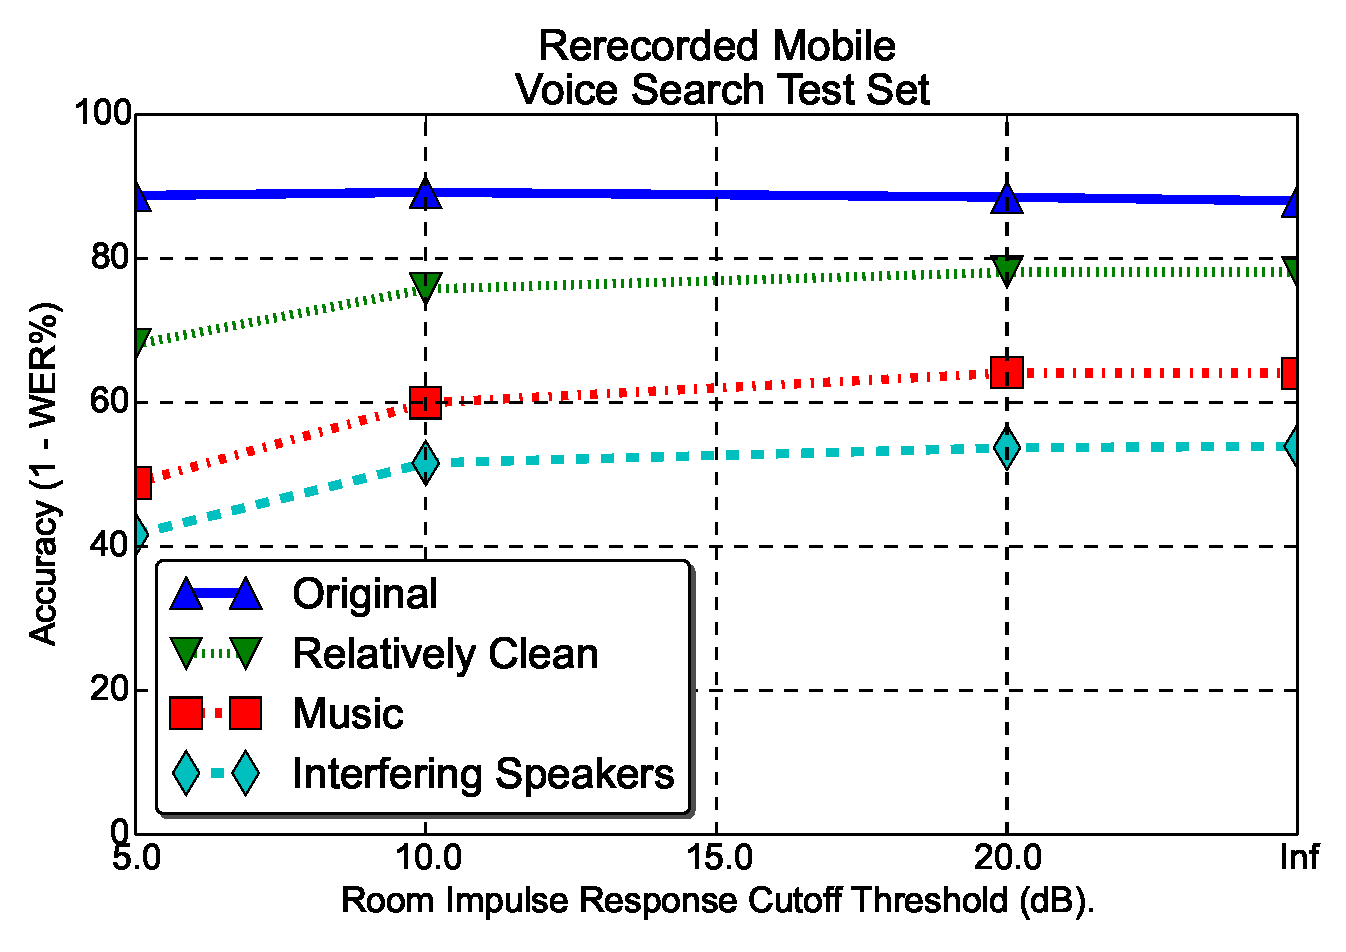
\includegraphics[width=70mm]{rir_cutoff_rerecorded_sets}
%      \label{fig:rir_cutoff_rerecorded_sets}
%    }
%    \vspace{-4mm}
%    \caption {
%      Word Error Rates (WERs) for the voice search test set 
%      at different reverberation time corrupted by (a) an
%      interfering speaker and (b) various noise in the 
%      DEMAND noise database.
%    }   
%   \vspace{-7mm}
%  \end{center}
%\end{figure}
%
%
\begin{figure}
  \begin{center}
    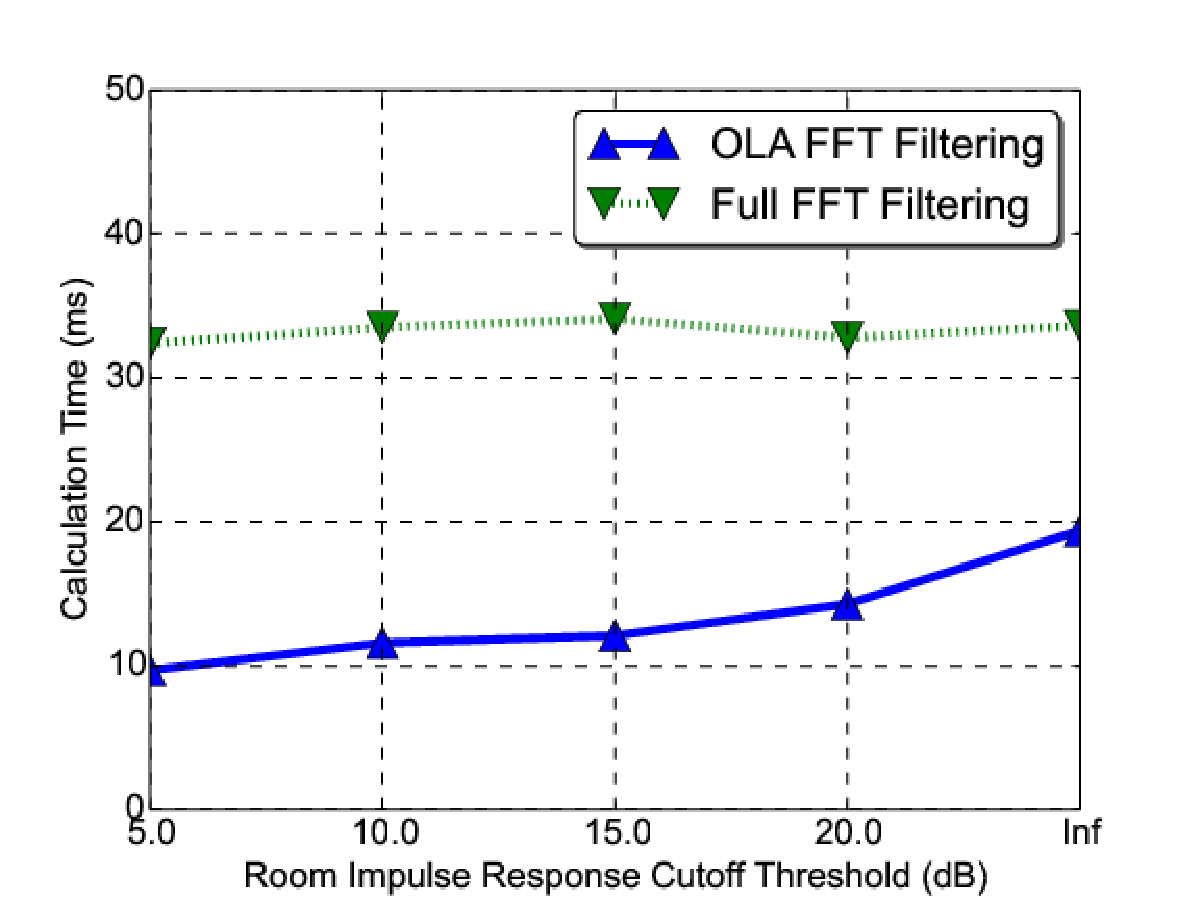
\includegraphics[width=70mm]{rir_cutoff_time}
    \caption {
      \label{fig:rir_cutoff_local_profiling}
      Profiling result on local desktop machine with
      different RIR cut-off threshold with and without
      OverLap Addition FIR filtering.
    }
  \end{center}
  \vspace{-7mm}
\end{figure}
%%   \vspace{-7mm}
%  \end{center}
%\end{figure}
\begin{table}%[!htbp]
  \renewcommand{\arraystretch}{1.3}
  \centering
  \caption{\label{tbl:local_machine_prof}The profiling result for processing a single utterance using
           the ``Room Simulator" on a local desktop machine}
\begin{tabular}{| c | c |}
  \hline
                         & \specialcell{Avg. Time per \\ Utterance (\textit{ms})} \\
   \hline
   \hline
  \specialcell{Original System \\
               \textit{Room Simulator} in \cite{C_Kim_INTERSPEECH_2017_1}}                            &  320.8 \textit{ms} \\
   \hline
  \specialcell{\texttt{FFTW3} Real FFT Filtering }                  &  44.2  \textit{ms} \\
   \hline
  \specialcell{OLA filtering }                             &  19.4  \textit{ms} \\
   \hline
  \specialcell{OLA filtering and 20 dB RIR cut-off}        &  14.3  \textit{ms} \\
  \hline  
\end{tabular}
\end{table}
%
%
%%
%
%
%
\begin{table*}%[th]
  \caption{\label{tbl:cpu_percentage} {The CPU usage portion of the FFT
          and \textit{Room Simulator} with the respect to the entire
          CPU pipeline in Fig. \ref{fig:gpu_cpu_structure}  and \\ relative
          speed up on \texttt{Google Borg} cluster \cite{A_Verma_eurosys_2015_1}.}}
  \vspace{2mm}
  \centerline{
    \begin{tabular}{| c | c | c | c | c | c | c |}
      \hline
            &  \specialcell{Original system}
            &  \specialcell{\texttt{FFTW3} OLA Filter   }
            &  \specialcell{\texttt{FFTW3} OLA Filter \\ with 20 dB RIR  Cut-off}
            &  \specialcell{\texttt{FFTW3} OLA Filter \\ with 10 dB RIR  Cut-off}  \\
      \hline \hline
      FFT portion (\%)       & 79.27 \%  &  10.11 \% &  \textbf{6.23} \% & 5.08 \% \\
      \hline
      \specialcell{Relative Speed Up \\ in FFT Portion (\%) }
                             &  -    & 34.0 times    &  \textbf{57.6 times} & 59.6 times       \\
      \hline \hline
      \specialcell{Entire Acoustic \\ Simulation (\%) }
                             & 80.01 \%  &  13.30 \% &  \textbf{9.69} \% & 8.05 \%  \\
      \hline
      \specialcell{Relative Speed Up \\ in Acoustic Simulation Portion (\%) }
                             &  -    &  26.1 times    &  \textbf{37.3 times}  & 45.7 times       \\
      \hline
    \end{tabular}
  }
\end{table*}
%
%
\begin{table*}%[th]
  \caption{\label{tbl:results} {Speech recognition experimental result in terms of Word Error Rates (WERs) \\
          with and without MTR using the room simulation system in \cite{C_Kim_INTERSPEECH_2017_1}  \\
          and different RIR cutoff thresholds.}}
  \vspace{2mm}
  \centerline{
    \begin{tabular}{| c | c | c | c | c | c | c |}
      \hline
            &  \specialcell{Baseline \\ without  MTR}
            &  \specialcell{MTR using  \\ One-time Batch \\ Room Simulation}
            &  \specialcell{Baseline   \\ (On-the-fly    \\ Room Simulation)}
            &  \specialcell{20 dB RIR  \\ Cut-off}
            &  \specialcell{10 dB RIR  \\ Cut-off}
            &  \specialcell{5 dB RIR   \\ Cut-off}  \\
      \hline \hline
      Original Test Set        & 11.70 \%   &  12.07 \% & 11.95 \%  & \textbf{11.43} \%  & 10.75 \% &  11.20  \%  \\
      \hline
      Simulated Noisy Set A    & 20.75 \%  &  15.58 \% & 14.88 \%  & \textbf{13.96} \% & 13.59 \%  &  14.99 \%  \\
      \hline
      Simulated Noisy Set B    & 50.78 \%  &  22.47 \% & 20.64 \%  & \textbf{19.58} \% & 21.37 \%  &   28.27 \%  \\
      \hline
      \specialcell{Device 1  } & 52.56 \%  &  22.39 \% & 21.69 \%  & \textbf{21.35} \% & 23.20 \%   &  29.53 \%  \\
      \hline
      \specialcell{Device 2  } & 51.59 \%  &  22.12 \% & 21.62 \%  &  \textbf{21.26} \% & 22.90 \%   & 29.39 \%  \\
      \hline
      \specialcell{Device 3  } & 54.89 \%  &  23.42 \% & 22.29 \%  &  \textbf{22.86} \%  & 26.47 \%  &  36.71 \%  \\
      \hline
      \specialcell{Device 3 \\ (Noisy Condition)  }
                              &  72.09 \%  &  36.21 \% & 35.88 \%  &  \textbf{35.83} \%  & 39.99 \%  &  51.11 \%  \\
      \hline
      \specialcell{Device 3 \\ (Multi-Talker Condition)  }
                             &  74.60 \%   &  47.63 \% & 46.03 \%  &  \textbf{46.21} \%  & 48.36 \%  & 58.31 \%   \\
      \hline
    \end{tabular}
  }
\end{table*}
%
%
%
%
%  fig.set_size_inches(10.0, 3.0)
%   bbox_inches='tight'
 
%
%
%\begin{subequations}
%  \begin{align}
%    \begin{split}
%      \mu_{\theta}^{o}[m] = \frac{\sum_{k \in \mathcal{K}^{o}}{p[m, k]\theta[m, \omega_k]}}
%          {\sum_{k \in \mathcal{K}^{+}}{p[m, k]}},
%    \end{split}
%    \\
%    \begin{split}
%      \sigma_{\theta}^{o}[m] = \frac{\sum_{k \in \mathcal{K}^{o}}{\theta[m, \omega_k]^2 p[m, k]}}
%          {\sum_{k \in \mathcal{K}^{o}}{p[m, k]}}
%          - \left( \mu_{\theta}^{o}[m] \right)^2,
%    \end{split}
%  \end{align}
%\end{subequations}
%$\mu_{\theta}^{-}[m]$ and $\sigma_{\theta}^{-}[m]$ are obtained in the same way:
%\begin{subequations}
%  \begin{align}
%    \begin{split}
%      \mu_{\theta}^{-}[m] = \frac{\sum_{k \in \mathcal{K}^{+}}{p[m, k]\theta[m, \omega_k]}}
%          {\sum_{k \in \mathcal{K}^{-}}{p[m, k]}},
%    \end{split}
%    \\
%    \begin{split}
%      \sigma_{\theta}^{-}[m] = \frac{\sum_{k \in \mathcal{K}^{-}}{\theta[m, \omega_k]^2 p[m, k]}}
%          {\sum_{k \in \mathcal{K}^{-}}{p[m, k]}}
%          - \left( \mu_{\theta}^{-}[m] \right)^2.
%    \end{split}
%  \end{align}
%\end{subequations}
%\subsection{Reliable Channel Mask Selection (RCMS)}
%\label{sec:RCMS}
%
%
\section{Experimental results}
\label{sec:experimental_results}
%
%
%
\begin{table}%[!htbp]
  \renewcommand{\arraystretch}{1.3}
  \centering
  \caption{Average $T_{60}$ Time of the Simulated Traing Set and
           Simulated Test Sets A and B.}
\begin{tabular}{| c | c | c | c |}
  \hline
                         & \specialcell{Simulated \\ Training Set}
                         & \specialcell{Simulated \\ Noisy Set A}
                         & \specialcell{Simulated \\ Noisy Set B}  \\
   \hline
  \specialcell{Average $T_{60}$ Time}
      & 0.482 \textit{s}
      & 0.167 \textit{s}
      & 0.479 \textit{s}\\
  \hline
\end{tabular}
\vspace{-7mm}
\end{table}
%
%
%\begin{figure}[tbp]
%  \begin{center}
%    \subfloat[] {
%      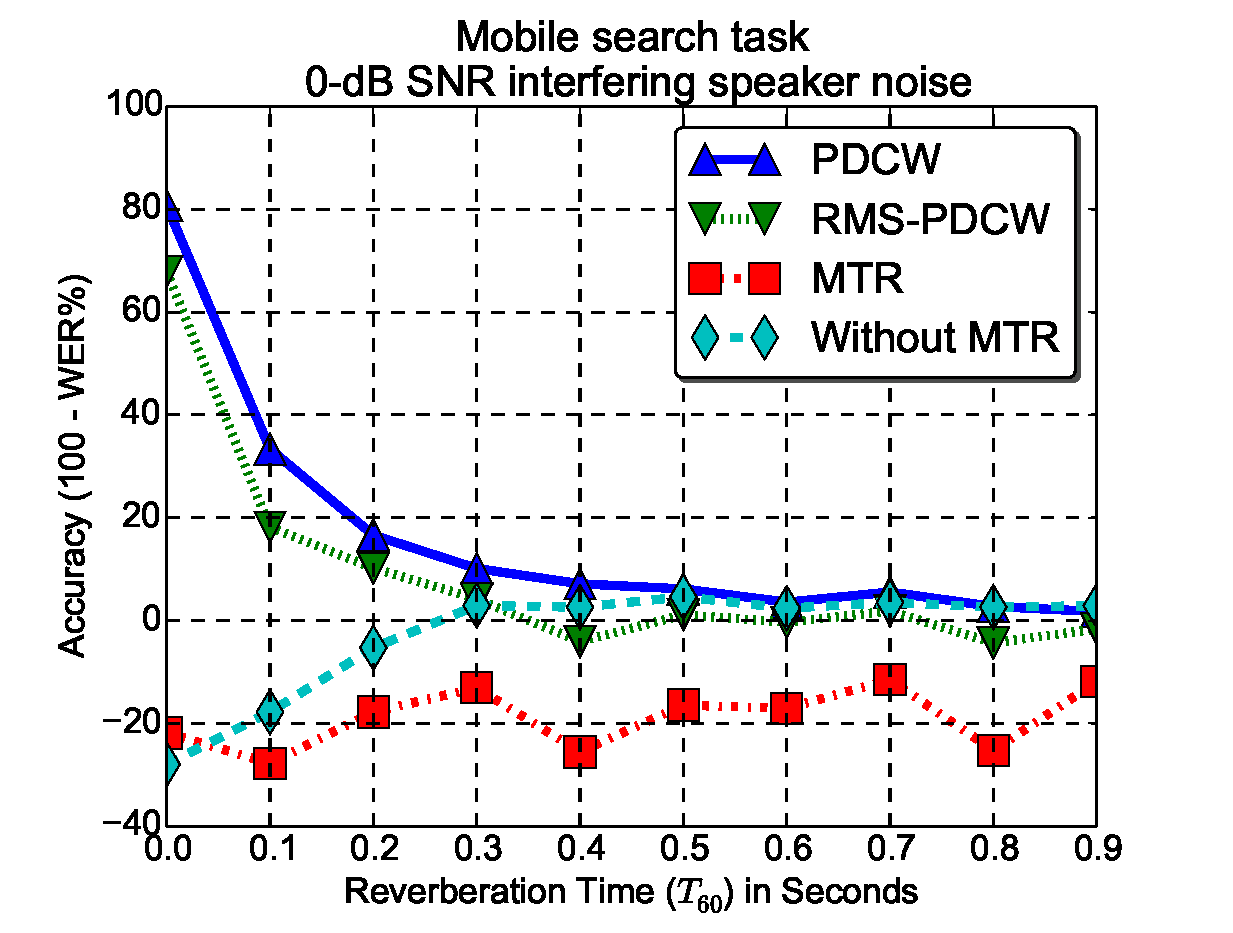
\includegraphics[width=70mm]{interfering_speaker_0db}
%      \label{fig:interfering_speaker_0db}
%    }
%    \\
%    \subfloat[] {
%      \label{fig:demand_noise_0db}
%      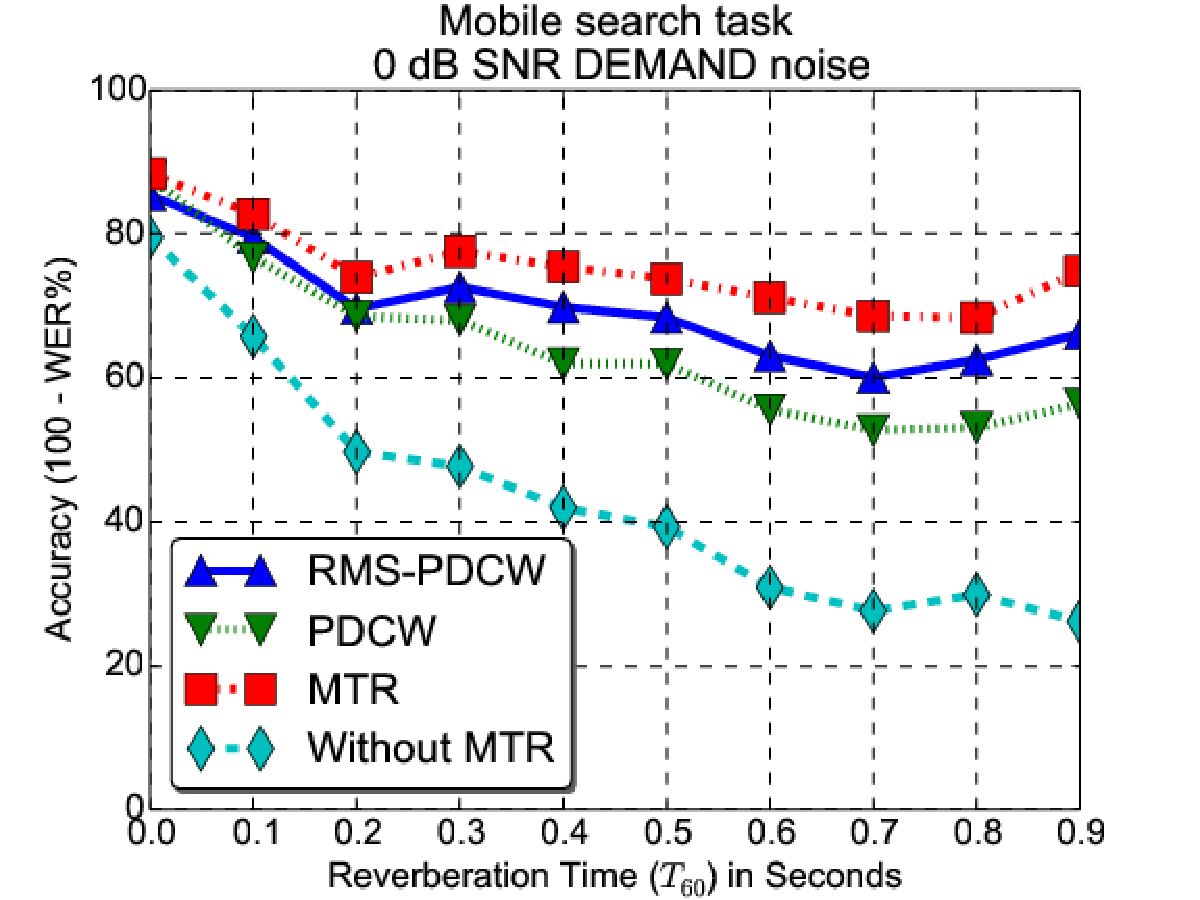
\includegraphics[width=70mm]{demand_0db}
%    }
%    \caption {
%      Word Error Rates (WERs) for the voice search test set
%      at different reverberation time corrupted by (a) an
%      interfering speaker and (b) various noise in the
%      DEMAND noise database.
%    }

%%
In this section, we present speech recognition results and CPU profiling
results obtained using \textit{Room Simulator} with different RIR cut-off
thresholds. For acoustic modeling, we use the structure shown in
% Is this the structure you used? I thought the model is plain lstm?
\AR{+1. I think these numbers are using logmel LSTMs? Clarify.}
\cite{B_Li_INTERSPEECH_2017_1}
%
with some modification.
One major difference is instead of generating two-channel simulated
waveform, we generate one-channel waveform \AR{Why? Maybe say for quicker turn around time?}.
We use the 128 dimension log-Mel feature whose window
size is 32 \textit{ms}. The interval between successive frame is 10
\textit{ms}. The low and upper cutoff frequencies of the Mel filterbank
are 125 \textit{Hz} and 7500 \textit{Hz} respectively.
Since it has been shown that long-duration features represented by overlapping
features are helpful \cite{H_Sak_INTERSPEECH_2015_1}, four frames
are stacked together and the input is downsampled by a factor of 3.
Thus we use a context dependent feature consisting of 512 elements
given by 128 (the size of the log-mel feature) x 4 (number of stacked frames).
The feature is processed by a typical multi-layer LSTM acoustic model.
We use 5-layer LSTMs with 768 units in each layer.
The output of the final LSTM layer is passed to a 768
unit DNN \AR{I don't think the model has DNNs. It's just a 5layer LSTM.}, followed by a softmax layer.
The softmax layer has 8192 nodes corresponding to the number of tied
context-dependent phones in our ASR system. The output state label is delayed
by five frames, since it was observed that
the information about future frames improves the prediction of the current frame
% This is not right reference for output delay, this is the one we used in speech team:
%\bibitem{sak2014long}
%H.~Sak, A.~W. Senior, and F.~Beaufays, ``Long short-term memory recurrent
%  neural network architectures for large scale acoustic modeling.'' in
%  \emph{Interspeech}, 2014, pp. 338--342.
%And if you want the main reference for delay in RNNs is Mike Schuster's paper:
%@article{schuster1997bidirectional,
%  title={Bidirectional recurrent neural networks},
%  author={Schuster, Mike and Paliwal, Kuldip K},
%  journal={IEEE Transactions on Signal Processing},
%  volume={45},
%  number={11},
%  pages={2673--2681},
%  year={1997},
%  publisher={IEEE}
%}
  \cite{H_Sak_INTERSPEECH_2014_1, M_Schuster_ieee_trans_signal_processing_1997}.
%
The acoustic model was trained using the Cross-Entropy (CE) loss
as the objective function, using precomputed alignments for utterance as targets.
To obtain results in Table \ref{tbl:results}, we trained for about 45 epochs.

For training, we used an anonymized and hand-transcribed
22-million English utterances (18,000-hr) set. The training set is the same as what we
used in \cite{B_Li_INTERSPEECH_2017_1, C_Kim_INTERSPEECH_2017_1}.
For evaluation, we used around 15-hour of utterances (13,795 utterances)
obtained from anonymized mobile voice search data. 
  We also generate noisy evaluation
sets from this relatively clean voice search data.
We use both simulated and rerecorded noisy sets.
Since our objective is deploying our speech recognition
systems on far-field standalone devices such as Google Home,
we rerecorded these evaluation sets using the actual hardware
in far-field environment.
Note that the actual Google Home hardware has two microphones
with microphone spacing of 7.1 cm. In our experiments in this section,
we selected the first channel out of two channel data.
 Three different devices
were used in rerecording, and each device was placed in five
different locations in an actual room resembling a real living
room. These devices are listed in Table 1 as ``Device 1'', ``Device 2'',
and ``Device 3''. As shown in Table \ref{tbl:results},
we observe that the RIR cut-off up to 20 \textit{dB} threshold does not
adversely affect the performance. However, if we cut the
RIR to 5 \textit{dB} threshold, then the performance under far-field
environment becomes significantly worse. This observation also confirms
that far-field speech recognition benefits from
RIRs with sufficiently long tails in the training set.
%
%
Table \ref{tbl:cpu_percentage} shows how much CPU resource was used
when training is done on \texttt{Google Borg} cluster
\cite{A_Verma_eurosys_2015_1} using the CPU/GPU
training architecture in Fig. \ref{fig:gpu_cpu_structure}. We observe that
if we use the \texttt{FFTW3}-based OLA filter using 20 \textit{dB} rir cutoff, we
may obtain 57.6 times speed-up in the FFT portion. The entire speed-up
of \textit{Room Simulator} portion is 37.3 times.
% 
\section{Conclusions}
In this paper, we describe how to efficiently implement
an acoustic room simulator to generate large-scale
simulated data for training deep neural networks.
We implement an efficient OverLap
Addition (OLA) based filtering using the open-source \texttt{FFTW3}
library. We investigate into the effects of the Room
Impulse Response (RIR) lengths. We conclude that we can cut
the tail portions of RIRs whose power is less than 20 \textit{dB}
below the maximum power without sacrificing speech recognition accuracy.
However, if we cut off RIR more than that, we observe it adversely
affects the performance for reverberant cases.
Using the approaches mentioned here, we could reduce the
room simulator portion in the CPU usage down to 9.69 \%
in CPU/GPU training architecture. Profiling result shows that
we obtain 22.4 times speed-up on a local desktop machine and 37.3 times
speed up on \texttt{Google Borg} cluster.
%
%\clearpage
%\newpage
%
\bibliographystyle{IEEEtran}
\bibliography{../../common_bib_file/common_bib_file}
%
%
\end{document}
